% =============================================================
%  ISY5002 -- Final Report
%  Traffic Monitoring and Forecasting from Singapore LTA Camera Images
%
%  Build:
%    latexmk -xelatex main.tex
%  Output:
%    build/main.pdf
% =============================================================

\documentclass[11pt,a4paper]{article}

% ---------------------------------------------------------------- fonts
\usepackage{fontspec}
\IfFontExistsTF{Arial}
  {\setmainfont{Arial}\setsansfont{Arial}}
  {\setmainfont{TeX Gyre Heros}\setsansfont{TeX Gyre Heros}}

% ---------------------------------------------------------------- page
\usepackage[a4paper,margin=1in]{geometry}
\usepackage{setspace}
\doublespacing
\setlength{\emergencystretch}{3em}

\usepackage{fancyhdr}
\setlength{\headheight}{14.5pt}
\pagestyle{fancy}
\fancyhf{}
\fancyfoot[R]{\thepage}
\renewcommand{\headrulewidth}{0pt}
\fancypagestyle{cover}{%
  \fancyhf{}%
  \renewcommand{\headrulewidth}{0pt}%
  \renewcommand{\footrulewidth}{0pt}%
}

% ---------------------------------------------------------------- layout
\usepackage{graphicx}
\usepackage{booktabs}
\usepackage[table]{xcolor}
\definecolor{oursrow}{HTML}{E6F3EC}
\usepackage{tabularx}
\usepackage{array}
\usepackage{float}
\usepackage{caption}
\usepackage{indentfirst}
\usepackage{enumitem}
\setlist{nosep}
\usepackage{csquotes}
\usepackage{xurl}

\captionsetup{font=small}
\graphicspath{{figures/}}
\renewcommand{\arraystretch}{1.05}
\setlength{\parindent}{0.5in}
\setlength{\textfloatsep}{8pt plus 2pt minus 2pt}
\setlength{\floatsep}{7pt plus 2pt minus 2pt}
\setlength{\intextsep}{8pt plus 2pt minus 2pt}

% ---------------------------------------------------------------- references
\usepackage[backend=biber,style=authoryear,sorting=nyt,giveninits=true,maxcitenames=2,maxbibnames=99]{biblatex}
\DeclareDelimFormat{nameyeardelim}{\addcomma\space}
\renewcommand*{\bibfont}{\footnotesize}
\setlength{\bibitemsep}{0pt}
\addbibresource{refs.bib}

% ---------------------------------------------------------------- links
\usepackage[hidelinks]{hyperref}
\hypersetup{
  bookmarksnumbered=true,
  bookmarksopen=true,
  pdftitle={Traffic Monitoring and Forecasting Workbench: A Modular Prototype},
  pdfsubject={ISY5002 Pattern Recognition Systems -- Final Report}
}

\begin{document}
\raggedbottom

\begin{titlepage}
  \thispagestyle{cover}
  \begin{singlespace}
    \centering
    \sffamily

    \vspace*{1.8cm}

    {\fontsize{12}{15}\selectfont
      ISY5002 Pattern Recognition Systems\par}

    \vspace{2.2cm}

    {\bfseries\fontsize{14}{18}\selectfont
      Traffic Monitoring and\\
      Forecasting Workbench:\\
      A Modular Prototype\par}

    \vspace{12pt}
    {\bfseries\fontsize{13}{16}\selectfont
      Final Report\par}

    \vspace{2.6cm}

    {\fontsize{10}{12}\selectfont Group Members:\par}
    \vspace{6pt}
    {\fontsize{12}{15}\selectfont
      \begin{tabular}{@{}l@{\hspace{2.2cm}}l@{}}
        Wang Mingyang & A0331532R \\
        Su Tanjia     & A0354250M \\
        Fu Junchun    & A0353395W \\
        Yan Yi        & A0333825A \\
        Wang Zimo     & A0328948J \\
      \end{tabular}\par}

    \vspace{1.8cm}

    {\fontsize{10}{12}\selectfont Submitted on\par}
    \vspace{4pt}
    {\fontsize{12}{15}\selectfont
      31 October 2026\par}

  \end{singlespace}
\end{titlepage}

\section*{Abstract}

Traffic monitoring observes road conditions; short-term forecasting anticipates
congestion. This project develops a modular prototype that evaluates the two
tasks on their respective data domains. A vehicle-recognition module fine-tunes
YOLO26m on MIO-TCD and 320 LTA images with teacher pseudo-labels, and is
evaluated on a leakage-aware MIO-TCD split, on LTA teacher agreement, and on a
63-image human-corrected subset of the week-2 validation frames. A per-camera
filter removes fixed false positives, and a stacked ensemble of detector counts,
background differencing and zero-shot CLIP assigns three congestion levels. A
forecasting module compares eight models on PEMSD8 under native and unified
nine-channel inputs, with five-seed checks for the leading four. A workbench
presents both source-labeled outputs.

On MIO-TCD, fine-tuning raises mAP@0.5 from 0.430 to 0.720. On the
human-corrected LTA subset, joint training lowers counting error and raises
recall but does not establish an mAP gain (0.478 versus 0.467). On PEMSD8, GWNET
has the lowest MAE; MultiHeadSTGCN is competitive but not superior. The filter
raises precision from 0.816 to 0.833 at a small recall cost; congestion
estimates agree with 74.3\% of 400 held-out labels. The prototype does not close
the loop from LTA images to local forecasting; calibrated time-aligned series
are still required.

\clearpage

\setcounter{tocdepth}{2}
\begin{singlespace}
\tableofcontents
\end{singlespace}
\clearpage

\section{Introduction}\label{sec:intro}

\subsection{Traffic Forecasting in Urban Mobility}\label{sec:intro-background}

Road transport is a major mode of movement in many cities, and the demand
placed on urban networks continues to grow with population and economic
activity. Congestion imposes costs on travelers, freight operators and the
environment, while the physical capacity of the road network is difficult to
expand in built-up areas. Operators therefore rely on traffic management to use
existing capacity efficiently. Short-term traffic forecasting is a core part of
this task: it estimates flow, occupancy or speed over the next 15 to 60 minutes,
giving signal controllers, route guidance systems, incident response teams and
network planners time to act before congestion forms.

Forecasting methods have developed alongside the sensing infrastructure that
supplies them. Loop detectors, radar and probe vehicles provide regular time
series at fixed locations, and early methods modeled each location
independently. As sensor networks expanded, spatio-temporal graph neural
networks became a prominent approach: they represent sensors as nodes in a graph
and learn both the spatial correlation between neighboring locations and the
temporal dynamics of the series \parencite{yu2018stgcn,wu2019gwnet}. Benchmarks such as LibCity
provide common data splits and implementations, making systematic comparison
possible \parencite{wang2021libcity,jiang2023libcity}.

Camera networks add a complementary view. Fixed roadside cameras cover wide
areas and record individual vehicles, and one-stage detectors can recover
vehicle positions and classes from each frame \parencite{ultralytics2026yolo}.
The resulting counts describe what is visible at the camera, while calibrated
flow, occupancy and speed series describe the aggregate traffic state used by
forecasting models. Combining the two views is a practical route toward
monitoring systems that both observe and anticipate traffic.

\subsection{Problem Statement and Project Scope}\label{sec:intro-objectives}

Singapore operates a dense network of fixed roadside cameras that provide
continuous visual coverage of its road network. The LTA collection used in this
project contains 15,316 images from eight cameras over two weeks, sampled at
ten-minute intervals. The images support vehicle recognition and manual
monitoring. They do not include calibrated flow, occupancy or speed at the
camera locations, and the ten-minute sampling interval gives a discontinuous
view of passing traffic. A forecasting model, by contrast, requires a regular
series of aggregate measurements. Public benchmarks provide such series, but for
different road networks.

The project addresses this mismatch by building a prototype with three
components: a vehicle recognition module, a traffic forecasting module and the
Traffic Monitoring and Forecasting Workbench. The detection module is trained on
MIO-TCD and jointly fine-tuned on LTA images with teacher pseudo-labels. The forecasting module is trained and
evaluated on PEMSD8 under a common protocol that compares eight models. The
workbench presents the outputs of both modules and labels their data sources. The
design keeps the two data domains explicit and defines the interface through
which a calibrated local series would connect them.

The project pursues three questions:

\begin{itemize}
  \item How well does a detector trained on MIO-TCD transfer to LTA images,
        measured against teacher labels and against a human-labeled LTA test
        set?
  \item How do representative forecasting models compare on PEMSD8 under a
        common protocol, and how does the custom model perform against them?
  \item How can a workbench present both outputs while keeping their data sources
        explicit?
\end{itemize}

The scope is limited to four vehicle classes in still images. Forecasting
focuses on traffic flow, with occupancy and speed as secondary analyses. The
project is a time-bounded prototype and pipeline design. It establishes the
processing chain, evaluation protocol and interface. An operational Singapore
forecasting system would additionally require calibrated sensing and longer
data collection. Nighttime LTA frames are a particular constraint: low light and
small vehicle scale make annotation difficult even for humans.

\subsection{Contributions}\label{sec:intro-contributions}

\begin{itemize}
  \item An LTA image set of 15,316 frames from eight Singapore cameras over two
        weeks, with a documented sampling and teacher pseudo-labeling pipeline,
        and a human-labeled test set of 63 week-2 images (1,197 boxes) frozen
        before evaluation.
  \item A leakage-aware MIO-TCD evaluation protocol based on scene groups, and
        a joint fine-tuning procedure that trains a COCO-pretrained YOLO26m on
        MIO-TCD and LTA images with teacher pseudo-labels; the model is applied
        to the full LTA collection.
  \item A per-camera false-positive filter calibrated by hand for all eight
        cameras, and a congestion-level estimate for all 15,316 LTA frames that
        combines the detector, a classical vision method and a zero-shot
        vision-language model; both are evaluated against human labels, with
        method selection and testing kept on separate label sets.
  \item A common-protocol benchmark of eight forecasting models on PEMSD8,
        covering native and unified nine-channel inputs, with five-seed paired
        checks for the top four models.
  \item MultiHeadSTGCN, an STGCN-based model with direct multi-step output,
        calendar inputs and a selectable spatial operator, examined in a staged
        ablation and against the benchmark models.
  \item A web workbench that integrates overview, camera monitoring and
        forecast views, with historical replay, camera-reliability indicators
        and a threshold-based risk ranking, together with an integration design
        for a calibrated local series.
\end{itemize}

\section{Literature Review}\label{sec:literature}

Traffic monitoring systems combine sensing and prediction. This section reviews
the two lines of work that inform the prototype: vehicle detection in traffic
imagery and spatio-temporal traffic forecasting. It also covers the evaluation
practices used to compare the resulting models.

\subsection{Vehicle Detection in Traffic Imagery}\label{sec:literature-detection}

One-stage detectors are the usual choice for traffic imagery because a single
forward pass returns boxes and classes at near-real-time speed
\parencite{ultralytics2026yolo}. COCO-pretrained weights are a strong starting
point \parencite{lin2014coco}, but the COCO camera geometry differs from fixed,
high-mounted traffic cameras. MIO-TCD provides a traffic-specific benchmark with
137,743 human-labeled localization frames from thousands of traffic cameras
\parencite{luo2018miotcd}. When target-domain
labels are unavailable, pseudo-labeling is a common approach: a teacher model
labels unlabeled images, and a student is trained on the resulting hard labels
\parencite{lee2013pseudo}. When the same teacher also supplies the evaluation
reference, the resulting score measures agreement with the teacher; the LTA
results in this report are interpreted on that basis.

\subsection{Traffic Forecasting}\label{sec:literature-forecasting}

Spatio-temporal graph models are widely studied for road-network forecasting.
STGCN combines temporal convolution with graph convolution
\parencite{yu2018stgcn}; Graph WaveNet learns an adaptive adjacency and uses
dilated temporal convolutions \parencite{wu2019gwnet}; MTGNN learns a graph and a
multi-step curriculum \parencite{wu2020mtgnn}; AGCRN uses node-specific
embeddings instead of a fixed adjacency \parencite{bai2020agcrn}. LibCity
provides a common implementation and evaluation environment
\parencite{wang2021libcity,jiang2023libcity}. In comparative studies, the models
are often trained with different input channels, optimizers and early-stopping
rules, so an observed difference reflects both architecture and training
recipe. The eight models compared in this project span feed-forward, recurrent,
fixed-graph, learned-graph and node-embedding designs, which gives the benchmark
coverage of the main modeling families rather than a single architecture.

\subsection{Evaluation and Benchmarking}\label{sec:literature-evaluation}

Frames from the same camera are highly correlated, so random image-level splits
leak near-duplicates into the test set. We group images by scene before
splitting and resample whole groups for confidence intervals. Detection accuracy
is reported with COCO-style mAP \parencite{lin2014coco}; uncertainty is estimated
with bootstrap resampling \parencite{efron1993bootstrap}. Forecasting comparisons
are most informative when every model receives the same input information; the
benchmark therefore reports both native configurations and a unified
nine-channel setting.

\subsection{Synthesis and Research Gap}\label{sec:literature-gap}

Across these lines of work, detection and forecasting are usually evaluated on
different data representations: annotated images for recognition and calibrated
sensor series for forecasting. Detection studies also face a cross-camera
adaptation problem when the target cameras differ in viewpoint, scale and
lighting from the training benchmark. Forecasting comparisons add a second
problem: native configurations differ in input features and training recipes, so
a ranking mixes architecture with implementation choices. Monitoring
integration raises a third problem: the two components produce different
outputs, at different time scales, and their data domains must remain visible to
the user. These gaps motivate a modular prototype that evaluates each component
on its own domain, reports both native and unified-input forecasting
comparisons, and makes the boundary between the two data sources explicit in
the interface.

\section{System Design and Methodology}\label{sec:method}

\subsection{System Overview}\label{sec:method-architecture}

Figure~\ref{fig:architecture} shows the prototype architecture. The upper path
maps LTA camera images to a detection table and to the recognition
post-processing layers described in Section~\ref{sec:method-congestion}; the
lower path maps PEMSD8 time series to forecast metrics. Both outputs feed the Traffic Monitoring and
Forecasting Workbench, a web-based interface that presents an overview, a
monitoring view and a forecast view. The two paths use separate data domains:
LTA camera images for recognition and PEMSD8 road-network series for
forecasting; the workbench labels the source of each view.
Section~\ref{sec:method-integration} defines the interface for connecting the
modules on a calibrated local series.

\subsection{Vehicle Recognition Module}\label{sec:method-detection}

The detection module is trained on MIO-TCD and jointly fine-tuned on LTA camera
images. The target-domain set has 320 images: 240 from week~1 for training and
80 from week~2 for validation, stratified by camera and by Singapore-time
day/night. A larger COCO-pretrained detector, YOLO26x, generates pseudo-labels
for all 320 images at the original 1920-pixel resolution with a confidence
threshold of 0.3.

Fine-tuning uses YOLO26m at 736 pixels with batch size~8 for a fixed 30 epochs
on an Apple M4 Pro, with one run per recipe. Two recipes are compared: MIO-TCD
only, and MIO-TCD augmented with the 240 Singapore training images repeated
twice.

All models, including the 80-class COCO baseline, are scored by the same
four-class evaluator. The joint model is then run at 1280 pixels over all
15,316 images and writes the CSV tables consumed by the workbench.

\begin{figure}[htbp]
  \centering
  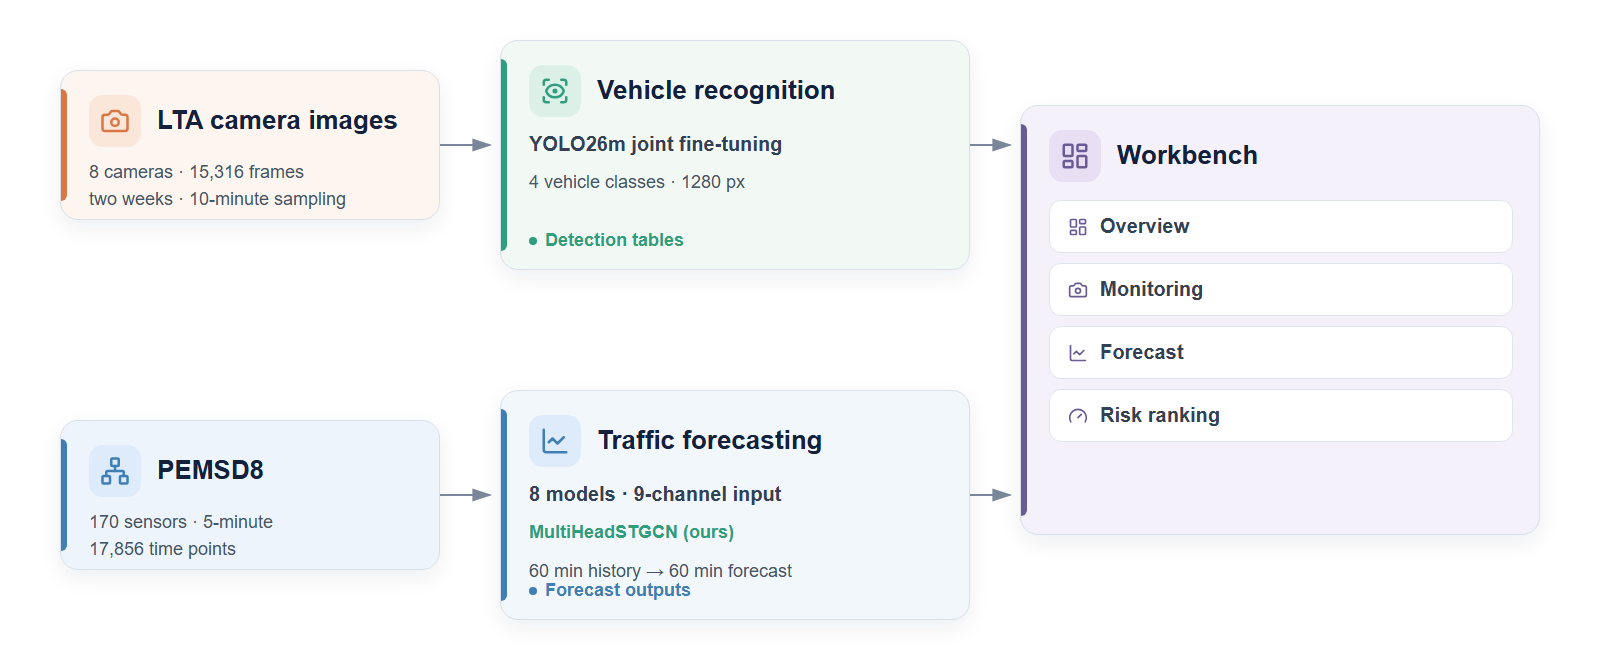
\includegraphics[width=\linewidth]{architecture.png}
  \caption{Prototype architecture. The upper path processes LTA camera images
  for vehicle recognition and its post-processing layers; the lower path
  processes PEMSD8 time series for traffic forecasting. Both outputs feed the
  workbench. The camera-filter and congestion layers are described in
  Section~\ref{sec:method-congestion} and omitted here for clarity.}
  \label{fig:architecture}
\end{figure}

\subsection{Camera Filter and Congestion Estimation}\label{sec:method-congestion}

The joint detector runs on fixed cameras, so many of its false positives recur
at the same image positions: road signs, traffic lights, lane markings and the
central median. A per-camera filter removes them without retraining. Each camera
is calibrated once with three elements in normalized image coordinates: a road
region, an exclusion set and detection zones. A box is kept only if its
bottom-centre point lies inside the road region. It is removed if it matches an
exclusion entry, either when its point lies in the entry (point rule) or only
when the whole box does (box rule), at all times or only by day or night. The
box rule protects vehicles that queue beside a fixed false positive; it is used
for a traffic light at camera 4703, where motorcycles wait next to it.

Calibration uses a browser page that plots the bottom-centre points of two weeks
of detections for each camera and proposes draft polygons from their density. An
annotator adjusts the vertices and accepts or rejects candidate false positives,
which are boxes that recur at the same position. The 80 week-2 validation images
are excluded from calibration, so the human-corrected images in
Section~\ref{sec:results-filter} were held out from calibration. Because the
filter is calibrated per camera, this evaluates image-level correction, not
transfer to new cameras. The filter can wrap the detector as a drop-in
replacement or filter the existing detection table.

The congestion module rates every LTA frame as free-flowing, moderate or
congested, judging only the detection zones: near-field segments that cover the
full width of one direction, drawn in the same calibration step. Three voters
score each frame independently. Voter~A uses the filtered output of the joint
detector: it counts vehicles whose bottom-centre lies in each zone and measures
box occupancy, the share of zone area covered by boxes. Voter~B is classical
image processing: for each camera and hour of day, a per-pixel median over two
weeks gives a background, and Canny edges \parencite{canny1986edge} present in
the frame but not in the background count as foreground, ignoring over-exposed
pixels. The background uses all frames in the collection, including test frames,
but no labels; it is an unsupervised, transductive step. Voter~C applies a
pretrained vision-language model without further
training: OpenCLIP ViT-B/16 trained on a LAION-2B subset of LAION-5B
\parencite{radford2021clip,cherti2023openclip,schuhmann2022laion} compares a
crop around the zones with three groups of text prompts, and its class
probabilities give a congestion score.

When a camera's zones cover two roads, the human label follows the more
congested one, so each voter is computed both over all zones and for the busiest
zone. Five candidate methods are compared: each voter alone with two cut points,
the median of the three voters' levels, and stacking
\parencite{wolpert1992stacking}, a multinomial logistic regression on the log
vehicle count, occupancy and the B and C scores. Features, cut points and the
primary method are chosen on practice labels only
(Section~\ref{sec:setup-metrics}); the frozen primary method then rates all
15,316 frames.

\subsection{Forecasting Module}\label{sec:method-forecasting}

The forecasting module operates on road-network time series. PEMSD8 provides a
calibrated multivariate benchmark with standard evaluation splits: 170 sensors,
five-minute observations, and flow, occupancy and speed measurements. The module
is trained, tested and compared on PEMSD8, which supports multivariate graph
models and comparison with published baselines. The LTA collection provides
per-frame vehicle counts at ten-minute intervals; Section~\ref{sec:method-integration}
defines the calibrated series required to connect these counts to the
forecasting module.

The module compares eight models under a common protocol: FNN, STGCN, MTGNN,
MultiHeadSTGCN, GRU, LSTM, GWNET and AGCRN. The first seven follow their LibCity
implementations; MultiHeadSTGCN is the project's custom model. The set covers
feed-forward, recurrent, fixed-graph, learned-graph and node-embedding designs.
Two input settings are compared: each model's default configuration, and a
unified nine-channel setting (flow plus time-of-day plus day-of-week). The
unified setting controls the information available to each model, but it does
not equalize optimizer, loss function, parameter count or training budget. The
top four models on the unified setting are re-run with seeds 0--4 and compared
with paired differences. Every run records its resolved configuration, data
provenance, training history and checkpoint selection.

MultiHeadSTGCN is based on STGCN and keeps its temporal and spatial blocks. It
changes four aspects. First, it predicts all output steps in one forward pass
instead of the LibCity STGCN implementation's single-step output followed by
autoregressive rolling. Second,
output heads are target-specific: each head produces the complete 12-step
horizon, and a single-target run uses one head. The multi-head capacity is
exercised only when several targets are trained jointly. The benchmark in this
report uses the single-target flow configuration, so its results do not
demonstrate a benefit from multiple heads. Third, it adds time-of-day and
day-of-week inputs. Fourth, it can use either Chebyshev convolution on the
symmetrized PEMSD8 sensor-link adjacency or directed dual-path propagation on
the original directed links. The default configuration uses the symmetric
Chebyshev variant, a collapsed output head that compresses the temporal axis
before the final projection, and the two calendar features.
Section~\ref{sec:results-ablation} quantifies each step.

\subsection{Workbench}\label{sec:method-workbench}

The Traffic Monitoring and Forecasting Workbench is a prototype traffic
monitoring and forecasting system. The product concept is a single operator
workbench that combines camera monitoring, vehicle counts and short-term
congestion forecasts in one interface. The prototype provides three views over
the processed outputs:

\begin{itemize}
  \item \textbf{Overview}: a situation summary, a needs-attention queue, camera
        and forecast health cards, and a camera coverage map.
  \item \textbf{Monitoring}: a camera picker, a time-controlled detection frame,
        camera reliability metrics (frames processed, zero-detection rate, mean
        confidence and completeness), and a per-class count timeline.
  \item \textbf{Forecast}: replay-time and horizon controls, a predicted-severity
        network schematic, an observed and forecast speed curve with an empirical
        residual band, and a threshold-based risk ranking.
\end{itemize}

Figure~\ref{fig:workbench} shows the overview: it combines the source labels for
both data domains, the needs-attention queue, the module health cards and the
camera coverage map. The workbench presents historical replay, and the interface
marks this state. It reads the detection tables and forecast run records, and each view labels
its data source. The Monitoring view shows
processed frames from the LTA collection; the Forecast view uses PEMSD8 and
identifies its sensors as belonging to a public California road network,
separate from the LTA cameras. The workbench is implemented as a lightweight web
application with static HTML, CSS and JavaScript for the interface and a Python
service for data access and consistency checks.

\paragraph{Congestion risk estimation.}
The Forecast view uses the speed-target run rather than the flow benchmark,
because the risk indicator is defined on speed. Detectors are classified as
watch below 55 mph, congested below 45 mph and severe below 35 mph. These
thresholds are operational choices anchored to a test-period free-flow median of
about 65 mph; they are not a traffic-engineering standard. For each detector, the
interface takes the worst predicted speed over the selected horizon, including
the current observation, and ranks detectors by severity, status and onset. The
result is a threshold-based risk indicator intended for comparative
visualization, not a validated congestion estimate. The shaded band is the
10th--90th percentile of per-detector residuals on the test period, an empirical
error range rather than a calibrated prediction interval.

\paragraph{Camera filter and congestion layers.}
The Monitoring view also shows two layers that read the outputs of
Section~\ref{sec:method-congestion}. A camera-filter switch dims the area outside
the road region, outlines the detection zones and draws the removed boxes with
their reason, and the reliability panel reports the share of boxes removed for
the camera. Each frame shows its congestion level, and a weekday-by-hour heatmap
gives the share of congested frames for the selected camera together with its
test-set accuracy. Without these outputs the view is unchanged. This congestion
level describes the LTA camera view; it is separate from the speed-based risk
indicator above, which is defined on PEMSD8.

\begin{figure}[t]
  \centering
  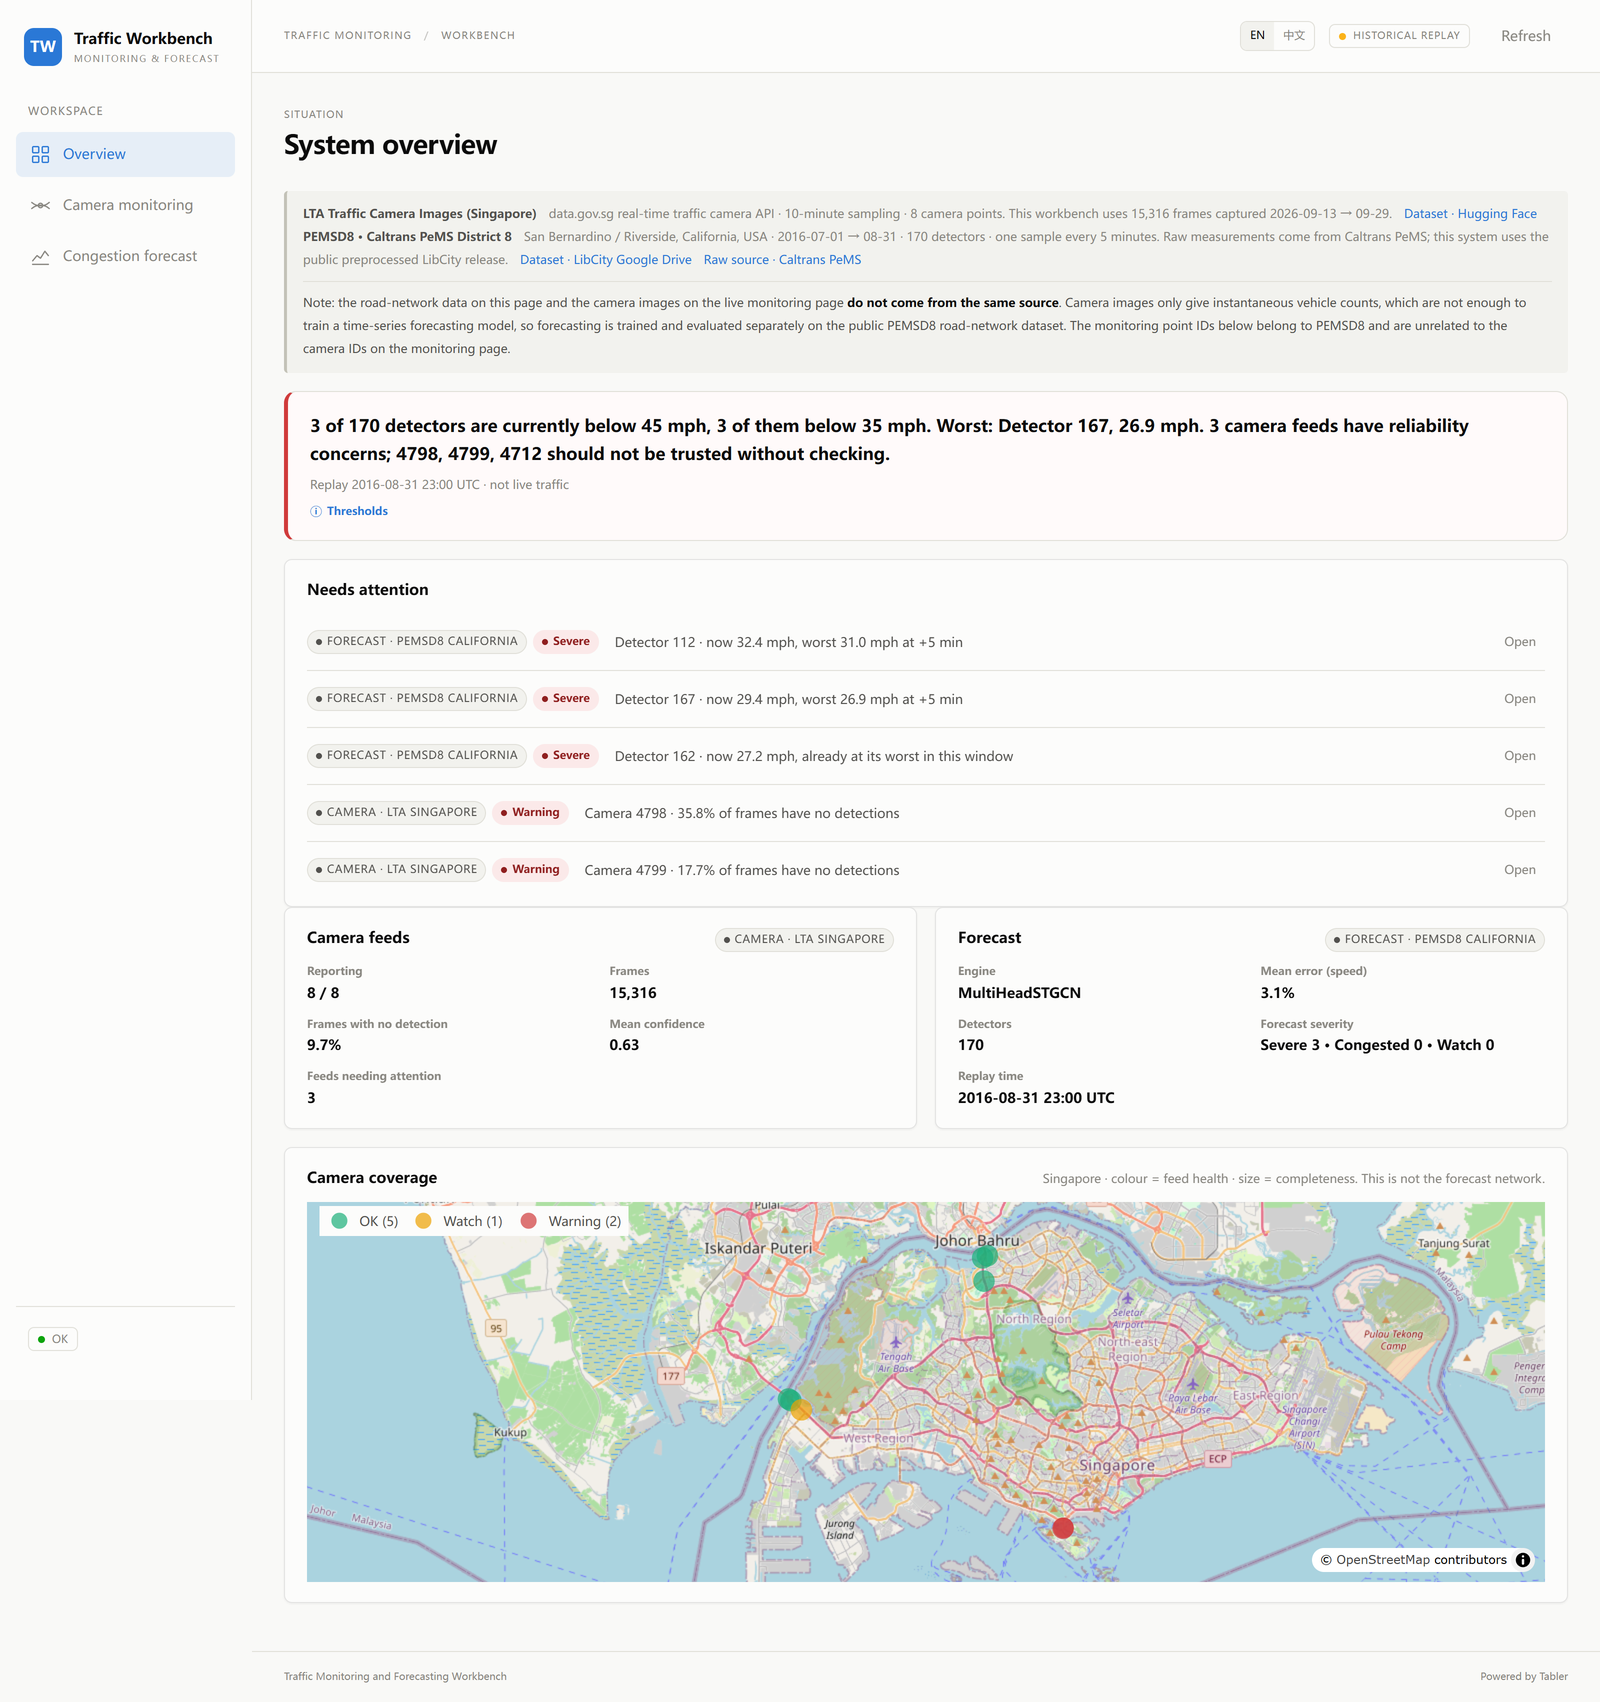
\includegraphics[width=0.92\linewidth]{workbench_overview.png}
  \caption{Workbench overview. Each view labels its data source. The page lists
  forecast and camera items that need attention, summarizes module health, and
  maps the eight LTA camera feeds.}
  \label{fig:workbench}
\end{figure}

\subsection{Implementation and Evaluation Tools}\label{sec:method-tools}

The detection module uses Ultralytics YOLO26 \parencite{ultralytics2026yolo} on
PyTorch \parencite{paszke2019pytorch}, with OpenCV and Pillow for image handling.
Fine-tuning and evaluation follow the MIO-TCD protocol
\parencite{luo2018miotcd}. The project code, workbench, experiment scripts and
run records are available in the repository.\footnote{The code revision used for
the reported runs is the \texttt{develop} branch:
\url{https://github.com/LOVEIII486/ISY5002-TrafficPrediction/tree/develop}}
The forecasting module uses LibCity \parencite{wang2021libcity,jiang2023libcity},
PyTorch, NumPy, pandas and SciPy.\footnote{LibCity code:
\url{https://github.com/LibCity/Bigscity-LibCity}} The workbench uses Python with
static HTML, CSS and JavaScript (Tabler components).\footnote{\url{https://tabler.io/}}
The camera filter and the congestion module use OpenCV, scikit-learn and
OpenCLIP \parencite{cherti2023openclip}.
Large prediction arrays and trained weights are not stored in version control;
the benchmark commands regenerate the arrays consumed by the workbench. The
human-corrected LTA annotations, manifests and COCO/YOLO exports are released in
\texttt{datasets/lta\_human\_v1}; images are referenced by filename and SHA-256
rather than redistributed. Detection accuracy is measured with COCO-style mAP
\parencite{lin2014coco}, and uncertainty is estimated with bootstrap resampling
\parencite{efron1993bootstrap}.

\subsection{Integration Design}\label{sec:method-integration}

The prototype is organized as three top-level modules with a shared workbench;
the camera filter and congestion estimate are recognition post-processing layers,
not additional data domains. A fully
integrated deployment requires a calibrated, time-aligned traffic series at the
camera locations. LTA images provide instantaneous vehicle counts; a forecasting
model additionally needs a consistent series of flow, and ideally occupancy and
speed, over weeks or months. The integration design has three steps. First,
calibrate camera counts against a trusted volume source and aggregate them to
fixed intervals. Second, obtain flow, occupancy and speed series for the same
locations and align their timestamps with the image feed. Where the existing
camera view is too distant or poorly lit, close-range cameras or dedicated
traffic sensors can provide clearer measurements. Third, train the forecasting
module on the local series and connect both modules to one data domain in the
workbench. This design defines the interface between the two modules
and the measurements required to complete it.

\section{Experimental Setup}\label{sec:setup}

\subsection{Datasets}\label{sec:setup-data}

The LTA collection contains 15,316 images from eight Singapore cameras over two
weeks, sampled at ten-minute intervals
\parencite{ltatrafficimages2026}.\footnote{The project image collection and the
human-corrected annotation subset are distributed as the
\href{https://huggingface.co/datasets/LOVEIII486/isy5002-lta-traffic-images}{LTA
image dataset on Hugging Face}; annotations are under
\texttt{annotations/lta\_human\_v1/}. The images remain under the Singapore Open
Data Licence 1.0; the annotations are released under CC BY 4.0.}
Week~1 and week~2 are disjoint in time.
For detection fine-tuning, 240 week-1 images are used for training and 80
week-2 images for validation, stratified by camera and by Singapore-time
day/night. The 240 training images also provide the pseudo-labeled
target-domain set used in joint fine-tuning. The labels are generated from
these images by YOLO26x; they are derived labels generated within the project.
Nighttime frames are a particular constraint: vehicles are small and poorly
lit, and even human annotation is difficult. Teacher labels and human labels
collected at night are therefore the least reliable reference.
Figure~\ref{fig:detection-examples} shows representative frames and labels from
both detection datasets.

MIO-TCD provides the human-labeled detection benchmark
\parencite{luo2018miotcd}.\footnote{The MIO-TCD localization dataset is
available at \url{https://tcd.miovision.com/}; paper DOI:
\url{https://doi.org/10.1109/TIP.2018.2848705}.}
Its localization set contains 137,743 annotated frames; the training release
used here contains 110,000 images. We map its eleven classes to four: work vans
to car; pickup, single-unit and articulated trucks to truck; bus and motorcycle
unchanged. Pedestrian, bicycle and non-motorized-vehicle boxes are dropped, and
images containing the class \texttt{motorized\_vehicle} (vehicles too small to
classify) are removed, leaving 89,701 images. Because many images are consecutive
frames from the same camera, we link images when they share a file hash, when
their 256-bit difference-hash distance is at most 16, when their background
thumbnails correlate at 0.95 or above, or when their vehicle-masked background
thumbnails correlate at 0.93 or above; connected components form 1,592 scene
groups. Whole groups are assigned to pools, and fixed-size samples are drawn
from the pools: 8,000 training images, 1,000 development images, 2,000 test
images and a 161-image motorcycle diagnostic split. The fixed caps keep the
30-epoch fine-tuning runs tractable and preserve rare-class coverage; the
remaining filtered images are not used. The test split contains 31 scene groups
and is evaluated once. Our splits are drawn from its training set; the official
test labels are not public.

PEMSD8 provides the forecasting benchmark: 170 sensors and 17,856 five-minute
observations. The series is distributed by LibCity \parencite{jiang2023libcity};
the raw measurements come from Caltrans PeMS.\footnote{Caltrans PeMS:
\url{https://pems.dot.ca.gov/}; LibCity dataset repository:
\url{https://github.com/LibCity/Bigscity-LibCity-Datasets}.}
The common protocol uses a 7:1:2 chronological split, 12 input steps and 12
output steps. The scaler is fitted on the training input windows, and the test
window indices are recorded for every run.
Figure~\ref{fig:pemsd8-series} shows a representative sensor series and its
daily profile.

COCO-pretrained weights provide model initialization. The datasets above supply
all training and evaluation data. Detection accuracy is measured on the
human-labeled MIO-TCD test set; on LTA, results are reported both against
teacher-generated labels and against human-corrected labels.

In addition, two human-annotated LTA sets are used. For detection accuracy and
the camera filter, an annotator corrected the boxes on the 80 week-2 validation
images; 17 images judged too difficult to label reliably were removed, leaving
63 images with 1,197 vehicle boxes. The annotations were initialized from
teacher pre-labels and are therefore human-corrected, not independent of the
teacher. For congestion, 600 frames
were labeled free-flowing, moderate or congested in a browser tool that outlines
the detection zones and hides the timestamp. The frames were drawn at random per
camera within five Singapore-time strata (weekday peak, weekday off-peak, weekend
day, evening and late night), never selected by any voter's score, and were split
before labeling into 25 practice and 50 test frames per camera. A frame skipped
as impossible to judge was replaced by a spare from the same camera and stratum.
The practice set contains 107 free-flowing, 47 moderate and 46 congested frames;
the test set contains 171, 127 and 102.

\begin{figure}[H]
  \centering
  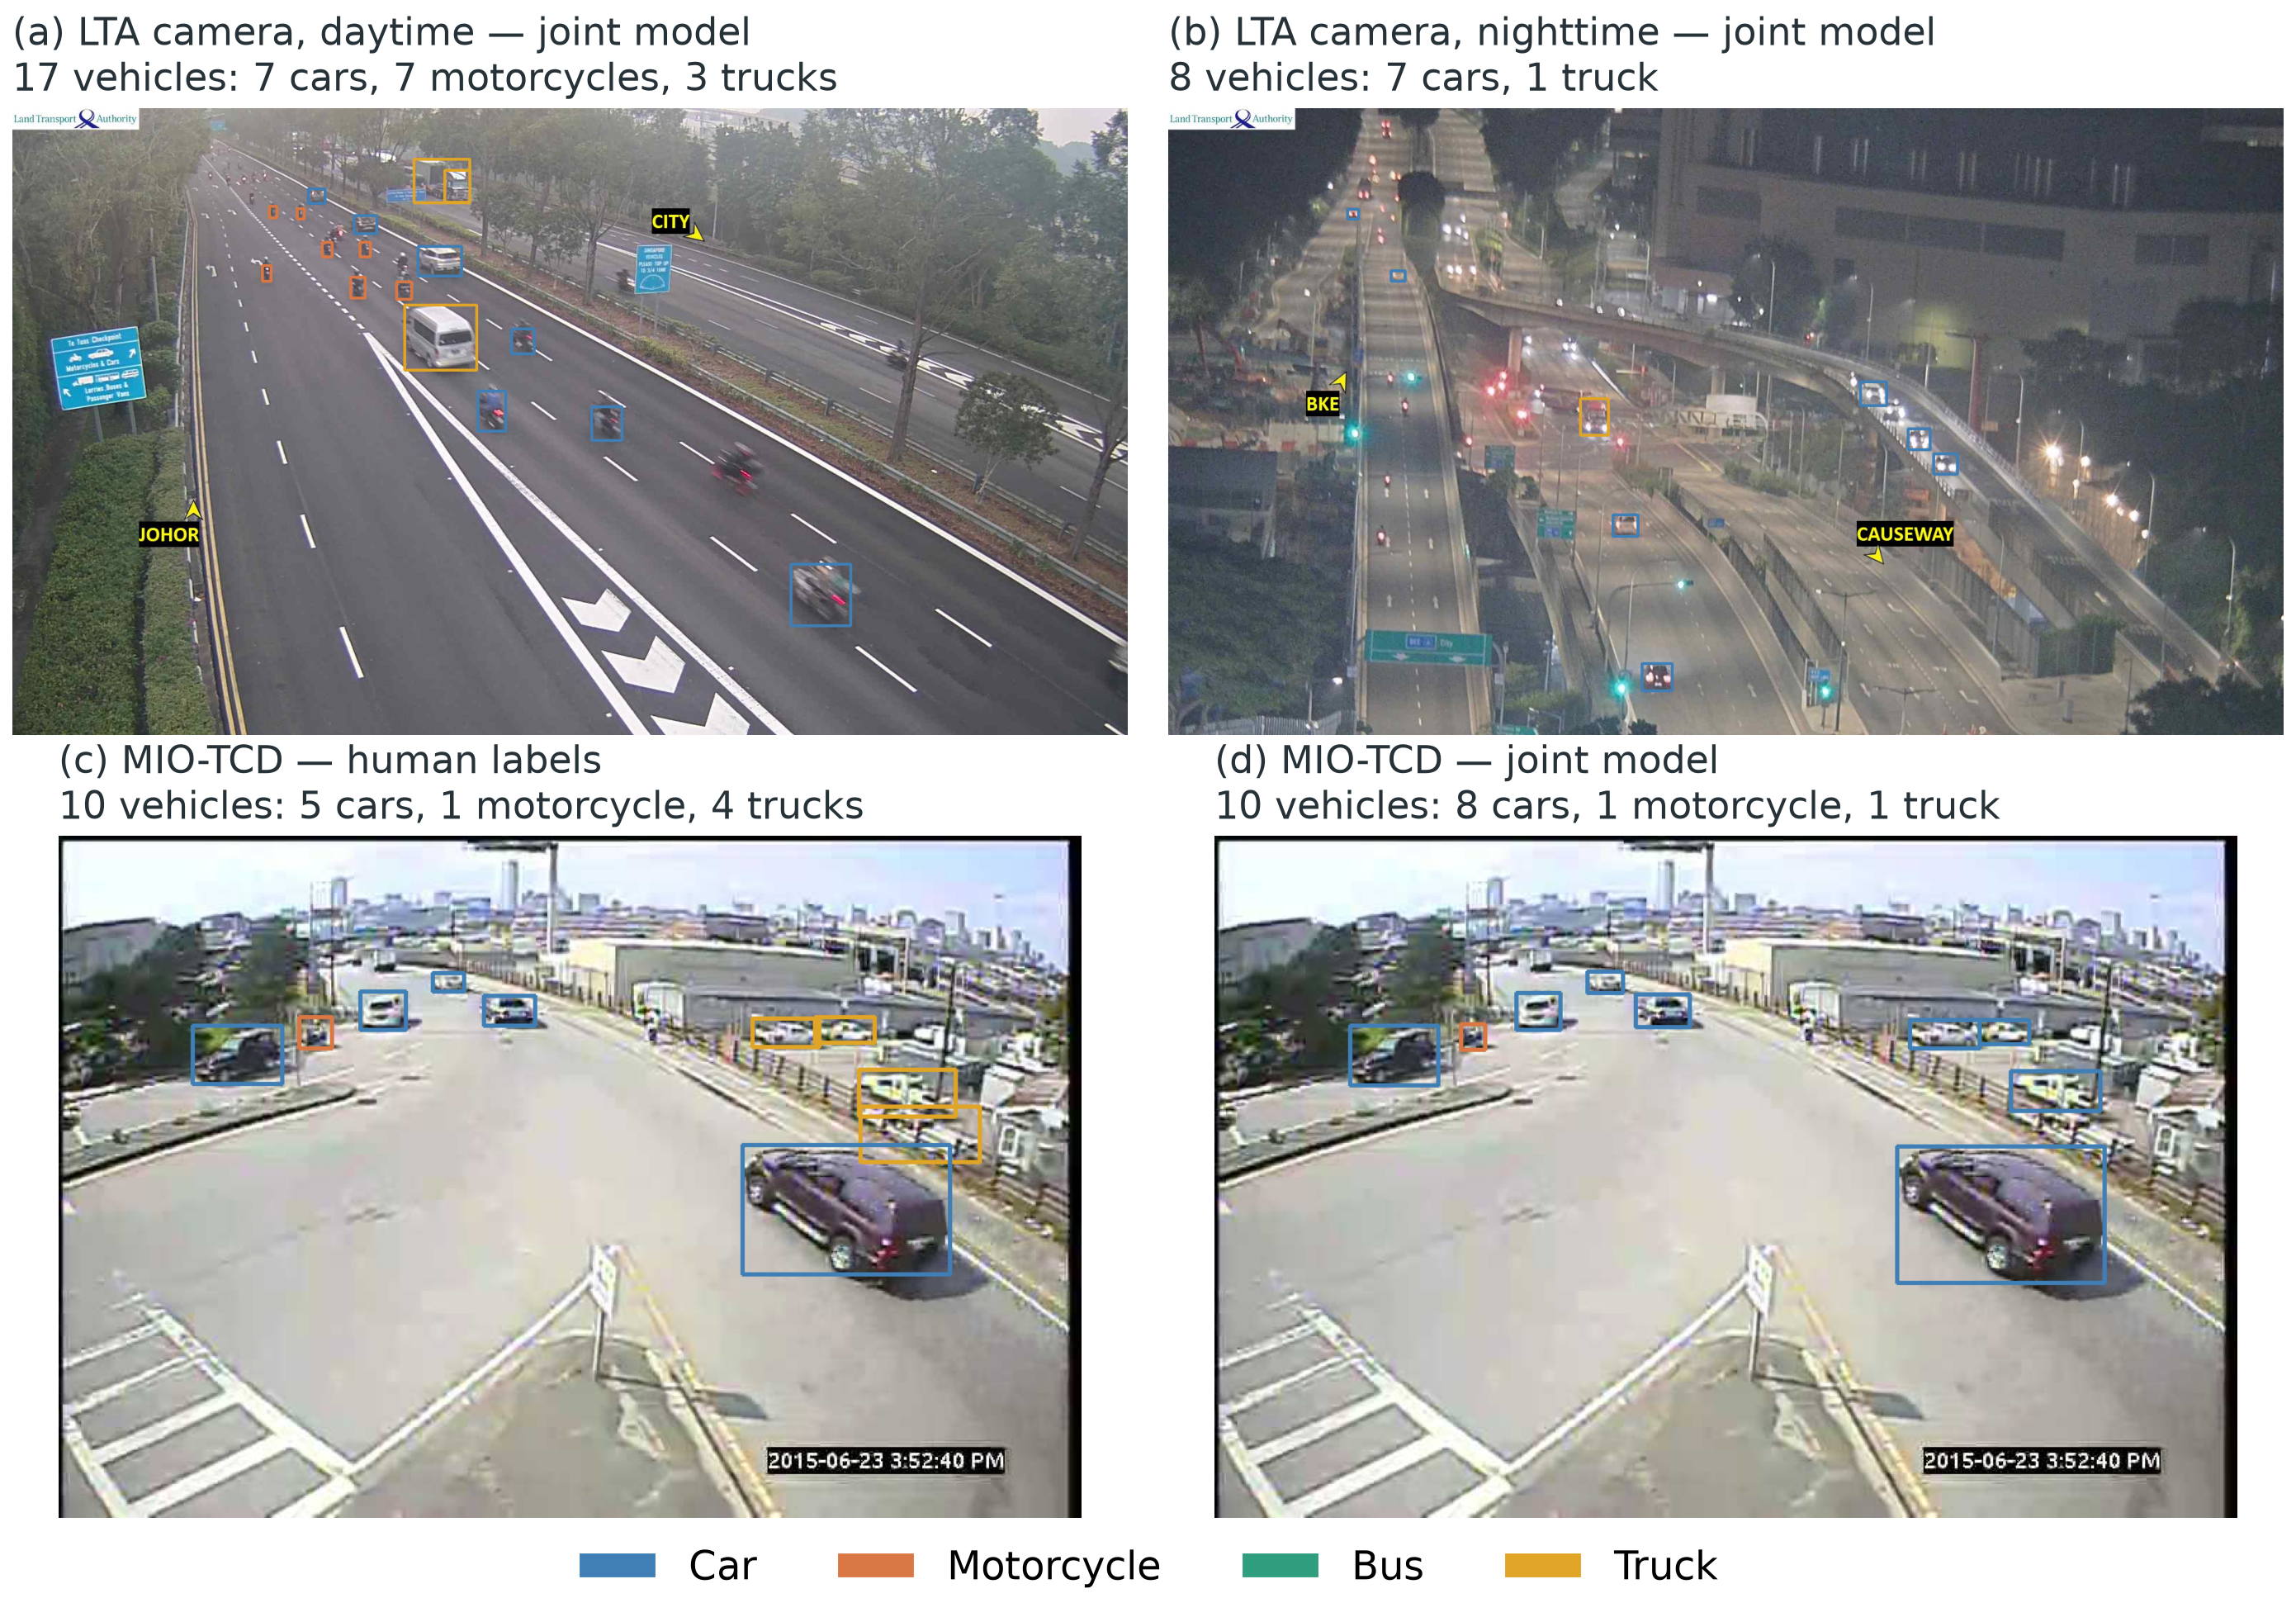
\includegraphics[width=0.92\linewidth]{detection_examples.png}
  \caption{Examples from the detection datasets. (a) LTA daytime and (b) LTA
  nighttime frames with joint-model detections; (c) a MIO-TCD test image with
  human labels; (d) the same image with joint-model detections. Box colors
  denote vehicle classes; titles report detected or labeled counts.}
  \label{fig:detection-examples}
\end{figure}

\begin{figure}[H]
  \centering
  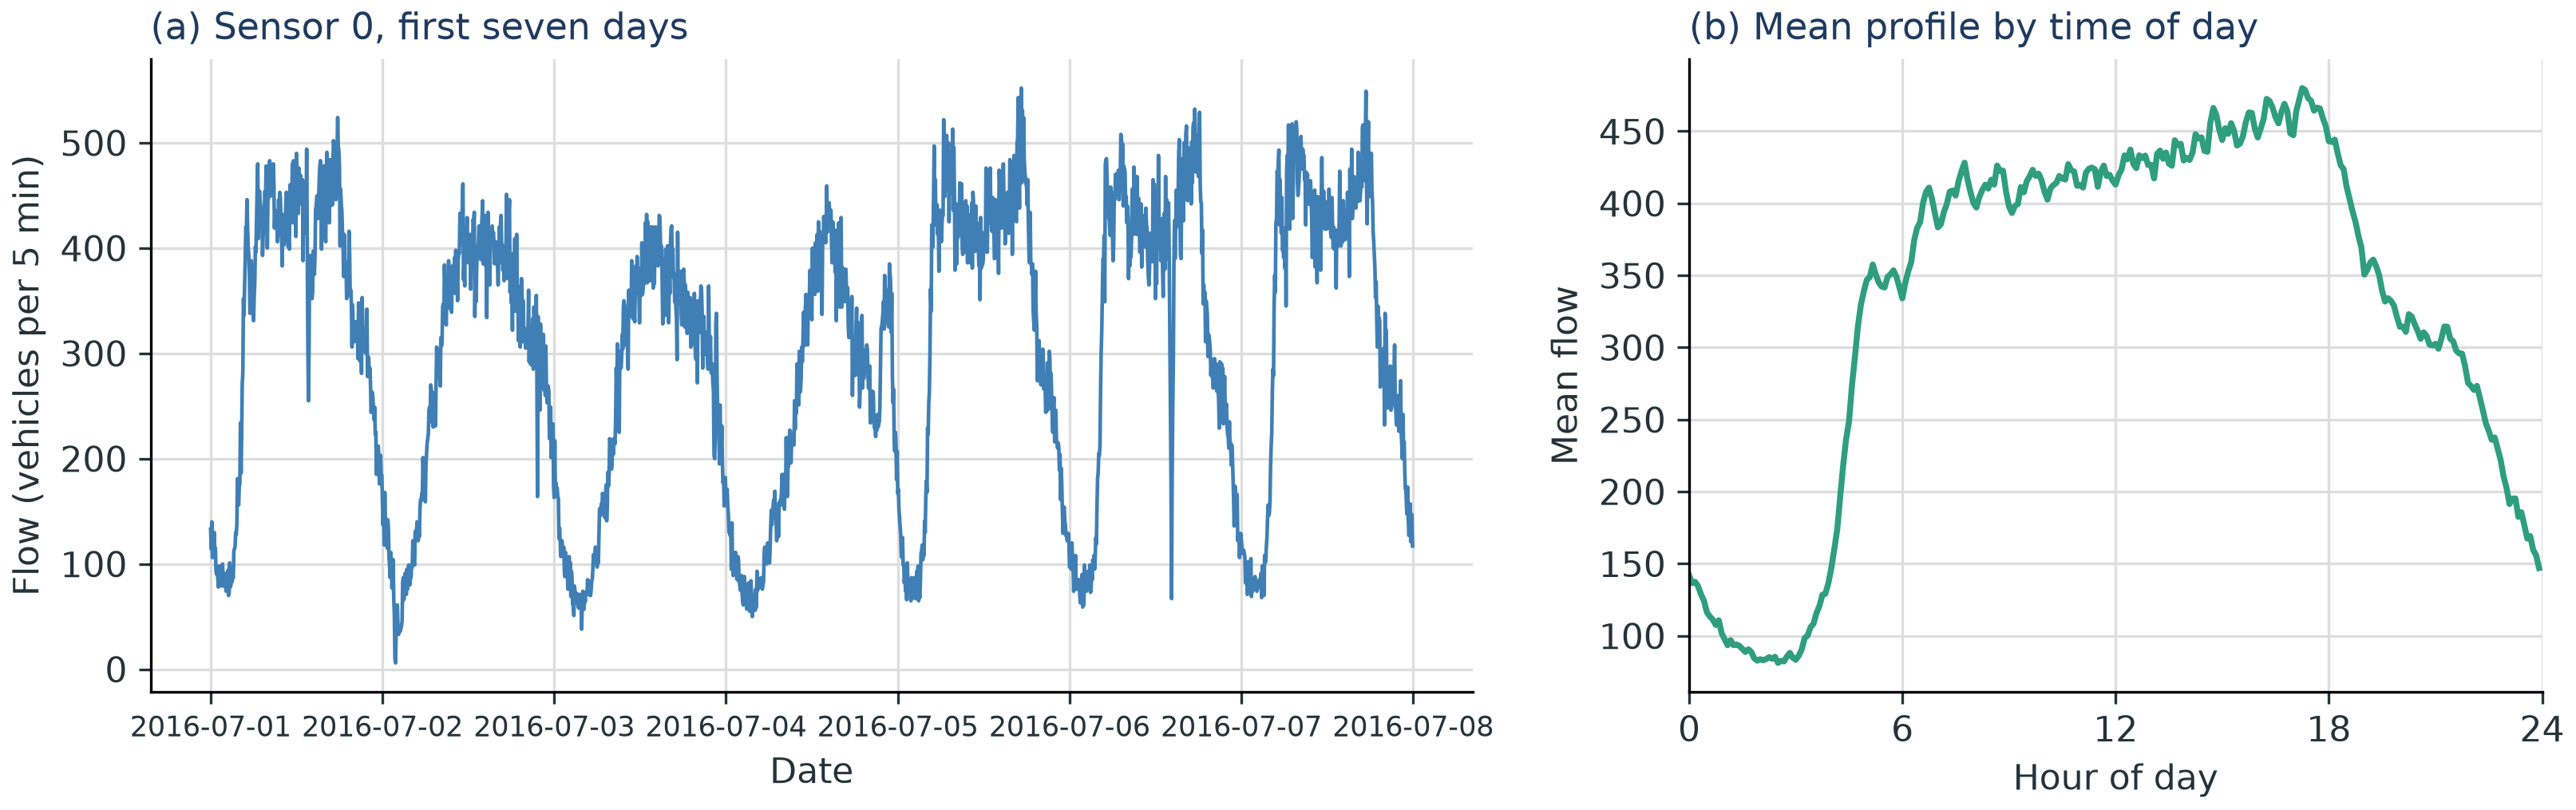
\includegraphics[width=\linewidth]{pemsd8_series.png}
  \caption{PEMSD8 traffic flow for sensor~0. (a) First seven days of the
  five-minute series; (b) mean flow by time of day over the full collection.
  The daily cycle motivates the time-of-day input used in the unified setting.}
  \label{fig:pemsd8-series}
\end{figure}

\subsection{Data Domains}\label{sec:setup-domains}

The prototype draws on two data sources. LTA images provide camera views and
per-frame vehicle counts. PEMSD8 provides calibrated flow, occupancy and speed
series for a road network. Each source supports one module: imagery for
recognition and calibrated series for forecasting. An end-to-end deployment
requires both at the same locations, aligned in time;
Section~\ref{sec:method-integration} defines this interface. The workbench presents
the two source-labeled views.

\subsection{Evaluation Protocol and Metrics}\label{sec:setup-metrics}

Detection is scored with COCO-style mAP \parencite{lin2014coco} at IoU~0.5 and
0.5:0.95, per-class AP, precision/recall at confidence~0.25, and mean absolute
counting error. Confidence intervals come from 2,000 bootstrap resamples of
scene groups; paired differences reuse the same resamples. This interval covers
scene sampling only, because each detector configuration was trained once.

The camera filter is scored on the 63 human-corrected images by class-agnostic
precision and recall at IoU~0.5 and confidence~0.25, before and after filtering,
with 2,000 bootstrap resamples of images. These intervals are image-level and do
not account for correlation between frames from the same camera, so they are
optimistic. Congestion levels are scored by
accuracy and linearly weighted Cohen's kappa \parencite{cohen1968kappa}, which
counts confusing free-flowing with congested as twice as severe as confusing
adjacent levels, together with precision and recall for the congested level.
Features, cut points and the primary method are chosen by five-fold
cross-validation repeated 20 times on the practice labels. The primary method is
the candidate with the highest cross-validated kappa; within 0.005 of the best,
the simpler candidate is preferred. The test labels are used once, after the
configuration is frozen, with 2,000 bootstrap resamples of test frames. These
intervals are frame-level; the 50 frames from each camera are correlated, so the
intervals are optimistic. Because peak hours are over-sampled, accuracy is also
reported with each test frame weighted by its camera and stratum's share of all
frames.

Forecasting uses masked MAE, RMSE and MAPE, averaged over the 12 output steps,
with 15/30/60-minute breakdowns at output steps 3, 6 and 12. MAE is measured in
vehicles per five-minute interval. Masked metrics ignore zero ground truth, with
a threshold of $10^{-4}$. The scaler is a standard scaler fitted on the training
input windows. All models use batch size 64, at most 100 epochs, early stopping
with patience 30, and checkpoint selection by validation loss; optimizer,
learning rate and schedule follow each model's LibCity default. Runs used
PyTorch on Apple MPS with LibCity commit \texttt{5a6391d}. Seeds control
initialization, shuffling and dropout, while data splits and test windows are
fixed. Forecast intervals are paired $t$-intervals over seeds, not bootstrap
intervals; the five-seed results are reported separately.

\section{Results and Analysis}\label{sec:results}

\subsection{Detection on MIO-TCD}\label{sec:results-detection}

Table~\ref{tab:det-test} reports the frozen test set. Fine-tuning raises
mAP@0.5 from 0.430 to 0.709 (MIO-only) and 0.720 (joint). The paired gains over
the pretrained detector are 0.279 and 0.291, with intervals that exclude zero.
No clear difference was established between the joint and MIO-only models on
this dataset (paired difference 0.011, 95\% CI −0.024 to 0.048). Counting error
roughly halves.
Figure~\ref{fig:detection-classes} gives the per-class breakdown.

\begin{table}[htbp]
  \centering
  \small
  \caption{Frozen MIO-TCD test set (2,000 images, human labels). mAP@0.5
  includes 95\% scene-group bootstrap intervals; other columns are point
  estimates.}
  \label{tab:det-test}
  \setlength{\tabcolsep}{3pt}
  \begin{tabular}{@{}lccccccc@{}}
    \toprule
    Model & mAP@0.5 & mAP@.5--.95 & Car & Moto. & Bus & Truck & Count MAE \\
    \midrule
    Pretrained YOLO26m & 0.429 (0.337--0.516) & 0.320 & 0.655 & 0.136 & 0.673 & 0.253 & 1.215 \\
    MIO-TCD only       & 0.709 (0.626--0.817) & 0.561 & \textbf{0.883} & 0.570 & \textbf{0.920} & \textbf{0.463} & \textbf{0.650} \\
    \rowcolor{oursrow}
    Joint fine-tuning  & \textbf{0.720} (0.645--0.825) & \textbf{0.563} & 0.874 & \textbf{0.646} & 0.908 & 0.453 & 0.698 \\
    \bottomrule
  \end{tabular}
  \par\smallskip
  \begin{minipage}{\linewidth}\footnotesize
    \textit{Note.} Bold marks the best value in each column; the shaded row is
    the joint model. The test set contains 33 motorcycle boxes; the motorcycle
    diagnostic split provides a larger sample.
  \end{minipage}
\end{table}

\begin{figure}[htbp]
  \centering
  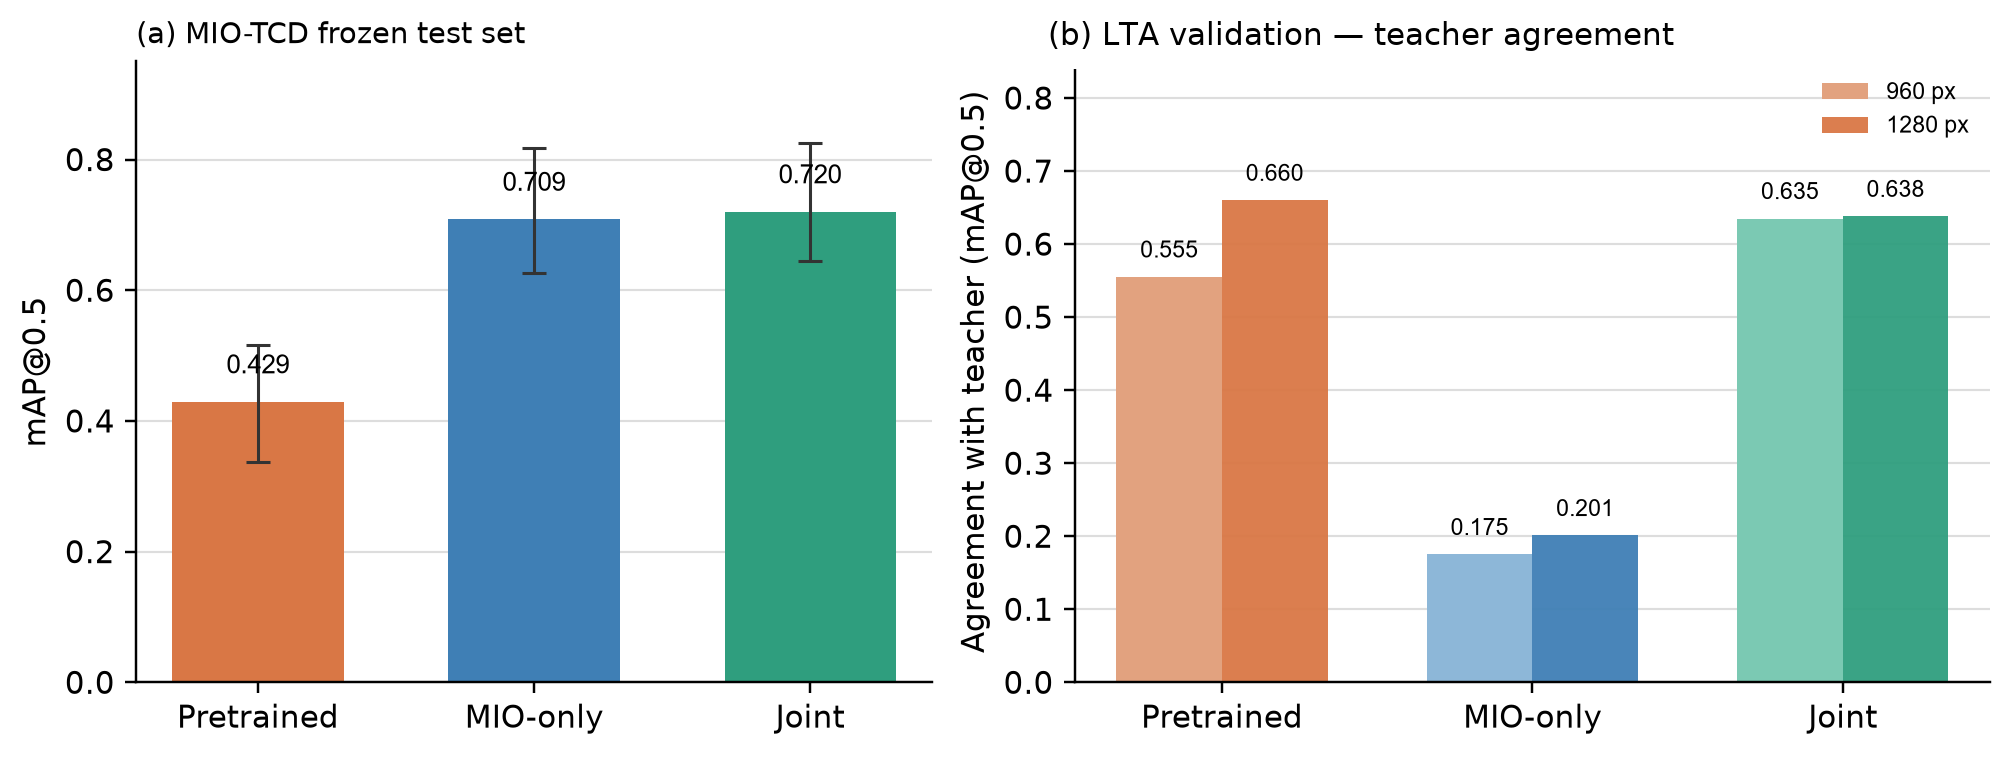
\includegraphics[width=0.96\linewidth]{detection_overall.png}
  \caption{Detection results. (a) Human-labeled MIO-TCD test set;
  (b) agreement with the YOLO26x teacher on LTA validation. The joint model is
  shown in green.}
  \label{fig:detection}
\end{figure}

\begin{figure}[htbp]
  \centering
  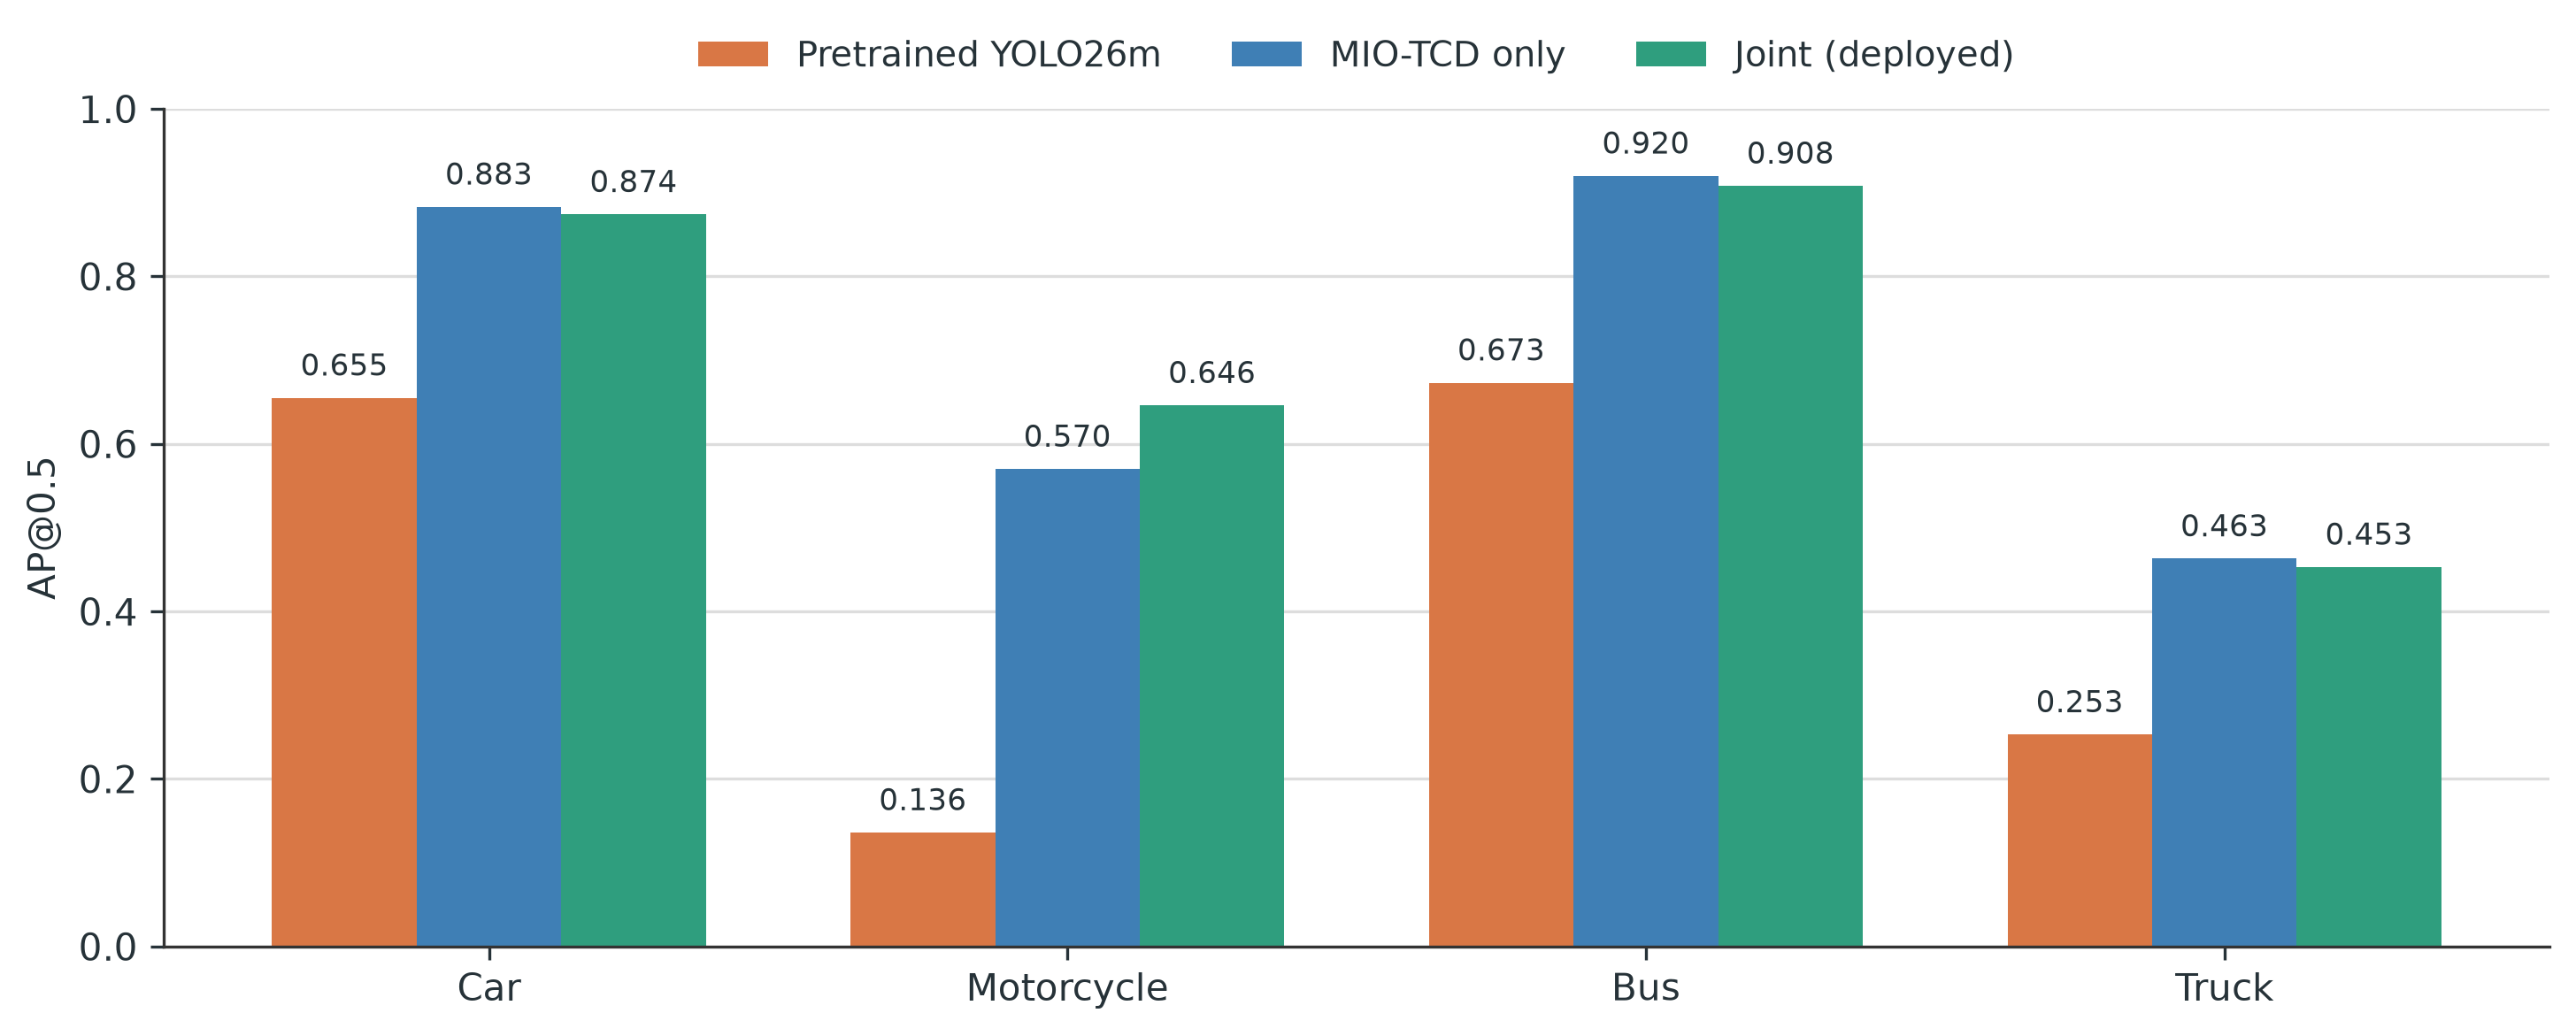
\includegraphics[width=0.96\linewidth]{detection_per_class.png}
  \caption{Per-class AP@0.5 on the frozen MIO-TCD test set. The joint model is
  shown in green and gives the largest gain on motorcycles.}
  \label{fig:detection-classes}
\end{figure}

\subsection{Cross-Domain Behavior on LTA}\label{sec:results-lta}

The LTA validation set uses the frozen YOLO26x pseudo-labels as its reference,
so the figures measure agreement with the teacher. The validation is evaluated
at 960 and 1280 pixels: 960 pixels is the lower-resolution setting used during
target-domain development, and 1280 pixels is the batch-inference resolution. At 960
pixels the pretrained model reaches 0.555, the MIO-only model 0.175, and the
joint model 0.635. The MIO-only result reflects the domain gap between North
American close-range views and the Singapore viewpoint.

At 1280 pixels, the batch-inference resolution, the pretrained model reaches
0.660 and the joint model 0.638. Agreement improves substantially over MIO-only
training, and the joint model's agreement is close to that of the pretrained
model at this resolution. The teacher row is a re-evaluation of YOLO26x at the
same inference resolutions after its labels were generated at 1920 pixels; it is
a reference point, not a mathematical upper bound on student performance.
Nighttime frames are the least reliable part of this proxy: low light and small
vehicle scale make both detection and manual annotation difficult. The
comparison is therefore a cross-domain proxy; accuracy across Singapore
traffic-camera conditions requires a human-labeled test set.
Figure~\ref{fig:model-comparison} gives a visual comparison on one frame. On
MIO-TCD the ranking reverses: MIO-only training reaches 0.709 mAP@0.5, compared
with 0.429 for the pretrained detector (Table~\ref{tab:det-test}). The joint
model is the compromise between the two domains.

\begin{table}[htbp]
  \centering
  \small
  \caption{LTA validation agreement with the frozen YOLO26x teacher (80 images,
  week~2).}
  \label{tab:lta}
  \begin{tabular}{@{}lccc@{}}
    \toprule
    Model & mAP@0.5 @960 & mAP@0.5 @1280 & Moto. AP@.5 @960 \\
    \midrule
    Pretrained YOLO26m & 0.555 & \textbf{0.660} & 0.539 \\
    MIO-TCD only       & 0.175 & 0.201 & 0.194 \\
    \rowcolor{oursrow}
    Joint fine-tuning  & \textbf{0.635} & 0.638 & \textbf{0.670} \\
    Teacher YOLO26x (re-evaluated) & 0.707 & 0.775 & 0.714 \\
    \bottomrule
  \end{tabular}
  \par\smallskip
  \begin{minipage}{\linewidth}\footnotesize
    \textit{Note.} Bold marks the best evaluated model in each column; the
    shaded row is the joint model. Teacher labels are model predictions. The
    teacher row re-evaluates YOLO26x at the same inference resolutions used for
    the students and serves as a reference, not an upper bound.
  \end{minipage}
\end{table}

\begin{figure}[H]
  \centering
  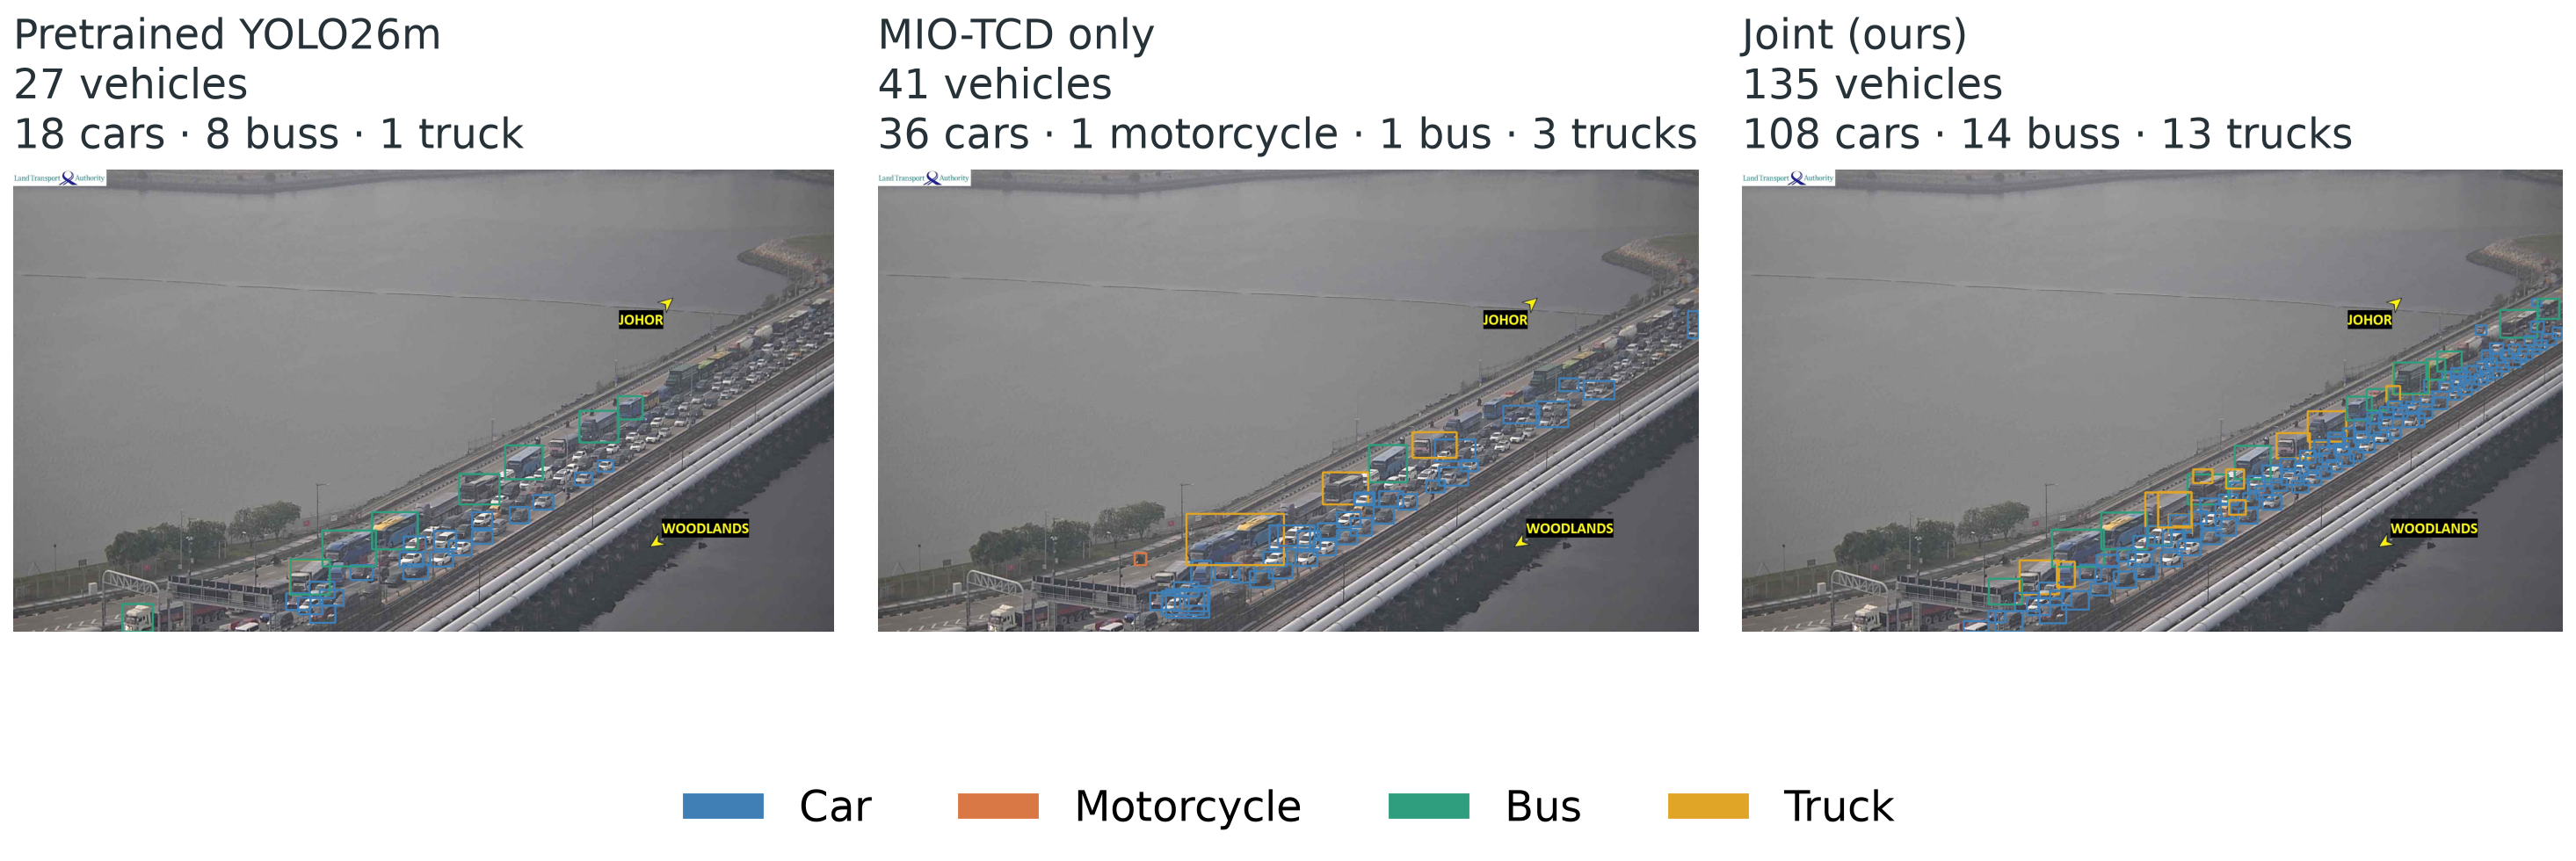
\includegraphics[width=\linewidth]{detection_model_comparison.png}
  \caption{Detection comparison on an LTA daytime frame (camera 2701, input
  1280, confidence 0.25). The pretrained detector finds 27 vehicles,
  MIO-TCD-only training 41, and joint fine-tuning 135. Box colors denote vehicle
  classes. The counts are model detections and illustrate detection density on
  one frame; they are not an accuracy measure. Table~\ref{tab:det-test} reports
  the quantitative comparison. On MIO-TCD the ranking reverses.}
  \label{fig:model-comparison}
\end{figure}

\subsection{Batch Inference on the LTA Collection}\label{sec:results-deployment}

The joint model was run over all 15,316 images at 1280 pixels with confidence
0.25. It produced 279,476 boxes: 187,928 cars, 41,109 motorcycles, 15,111 buses
and 35,328 trucks. The mean is 18.25 vehicles per frame, 27.22 during Singapore
daytime and 8.93 at night. A total of 1,478 frames returned zero detections,
1,437 of them at night. These frames are concentrated at night, where low light
and small vehicle scale limit both detection and manual verification. Nighttime
traffic volumes are also lower, so a zero-detection frame does not by itself
prove that vehicles were missed. The count is a detection count and may
understate nighttime traffic; the workbench's monitoring view presents it
alongside camera reliability indicators.

\subsection{Workbench}\label{sec:results-workbench}

The workbench presents the batch-inference outputs through three views. The
Overview view reports eight cameras, 15,316 processed frames, 279,476 detections
and the forecasting engine used for the speed target, together with camera and
forecast health and a needs-attention queue. The Monitoring view exposes
per-camera reliability (zero-detection rate, completeness and mean confidence), a
time-controlled detection frame and per-class counts. The Forecast view provides
replay-time and 15/30/60-minute horizon controls, a predicted-severity network
schematic, an observed and forecast speed curve with an empirical residual band,
and the threshold-based risk ranking defined in
Section~\ref{sec:method-workbench}. The interface marks the historical replay
state, and each view labels its data source; the Forecast view identifies PEMSD8
as a public California road-network dataset separate from the LTA cameras. The
service layer performs consistency checks against the recorded metrics and
reports warnings when output sets are incomplete or inconsistent.

\subsection{Forecasting: Eight-Model Comparison}\label{sec:results-forecast}

Table~\ref{tab:forecast-default} reports the default-configuration comparison.
GWNET has the lowest MAE among the evaluated configurations (14.648), followed
by MultiHeadSTGCN (14.839), MTGNN (15.106) and AGCRN (15.612). The configurations differ in input channels and
training recipes, so the table compares complete methods under the repository's
public protocol. The graph column distinguishes models that use the fixed road
adjacency from those that learn a graph or node embeddings.

\begin{table}[htbp]
  \centering
  \small
  \caption{Eight-model forecasting comparison on PEMSD8 traffic flow, default
  configuration, seed~0.}
  \label{tab:forecast-default}
  \begin{tabular}{@{}llcccc@{}}
    \toprule
    Model & Graph & Input channels & MAE & RMSE & MAPE (\%) \\
    \midrule
    GWNET                & Learned graph & 1 & \textbf{14.648} & \textbf{23.504} & \textbf{9.78} \\
    MTGNN                & Learned graph & 2 & 15.106 & 23.756 & 10.53 \\
    \rowcolor{oursrow}
    MultiHeadSTGCN & Road adjacency & 9 & 14.839 & 23.614 & 9.91 \\
    AGCRN                & Learned embeddings & 1 & 15.612 & 24.474 & 10.31 \\
    STGCN                & Road adjacency & 1 & 17.436 & 26.577 & 10.96 \\
    GRU                  & None & 2 & 19.706 & 32.363 & 12.27 \\
    FNN                  & None & 1 & 21.246 & 32.461 & 13.30 \\
    LSTM                 & None & 2 & 21.779 & 36.121 & 13.24 \\
    \bottomrule
  \end{tabular}
  \par\smallskip
  \begin{minipage}{\linewidth}\footnotesize
    \textit{Note.} Bold marks the lowest error in each column; the shaded row is
    the project's model. Road adjacency is the symmetrized PEMSD8 sensor-link
    graph; learned graphs and embeddings are estimated from data. Native input
    channels: 1 = flow; 2 = flow + time-of-day; 9 = flow + time-of-day + seven
    day-of-week one-hot features. MAE is in vehicles per five-minute interval.
    Default configurations also differ in training settings; this is a
    complete-method comparison.
  \end{minipage}
\end{table}

\subsection{The Custom Model: Ablation and Comparison}\label{sec:results-custom}

MultiHeadSTGCN is built on STGCN and keeps its temporal and spatial blocks. The
ablation ladder changes one design choice at a time within the custom
implementation, but the reference STGCN is the LibCity implementation. The two
also differ in training loss (masked MSE for STGCN, masked MAE for the custom
model), input features and multi-step strategy. The ladder therefore measures
the combined effect of the listed choices, not an isolated architecture effect.

Direct multi-step output lowers MAE from 17.61 to 16.05 (8.9\%). Adding
time-of-day and day-of-week lowers it to 15.00, an additional 6.5\% and a
cumulative 14.8\% relative to 17.61; day-of-week alone has little effect, while
the combination with time-of-day is stronger than either feature alone.
Chebyshev convolution on the symmetrized road adjacency lowers MAE to 14.90
(0.7\%); this difference is close to the 0.5\% variability observed when the same
configuration is rerun, so it is an observation rather than a stable gain. The
directed dual-path variant gives 14.91. Figure~\ref{fig:ablation} summarizes the
ladder.

Three comparisons should be kept separate. In the default-configuration
benchmark, STGCN (17.44) and MultiHeadSTGCN (14.84) differ by 14.9\%. In the
unified nine-channel benchmark, STGCN (16.11) and MultiHeadSTGCN (14.84) differ
by 7.9\%. The staged ablation above uses a different STGCN reference (17.61).
These are complete-recipe comparisons and are not interchangeable.

\begin{figure}[htbp]
  \centering
  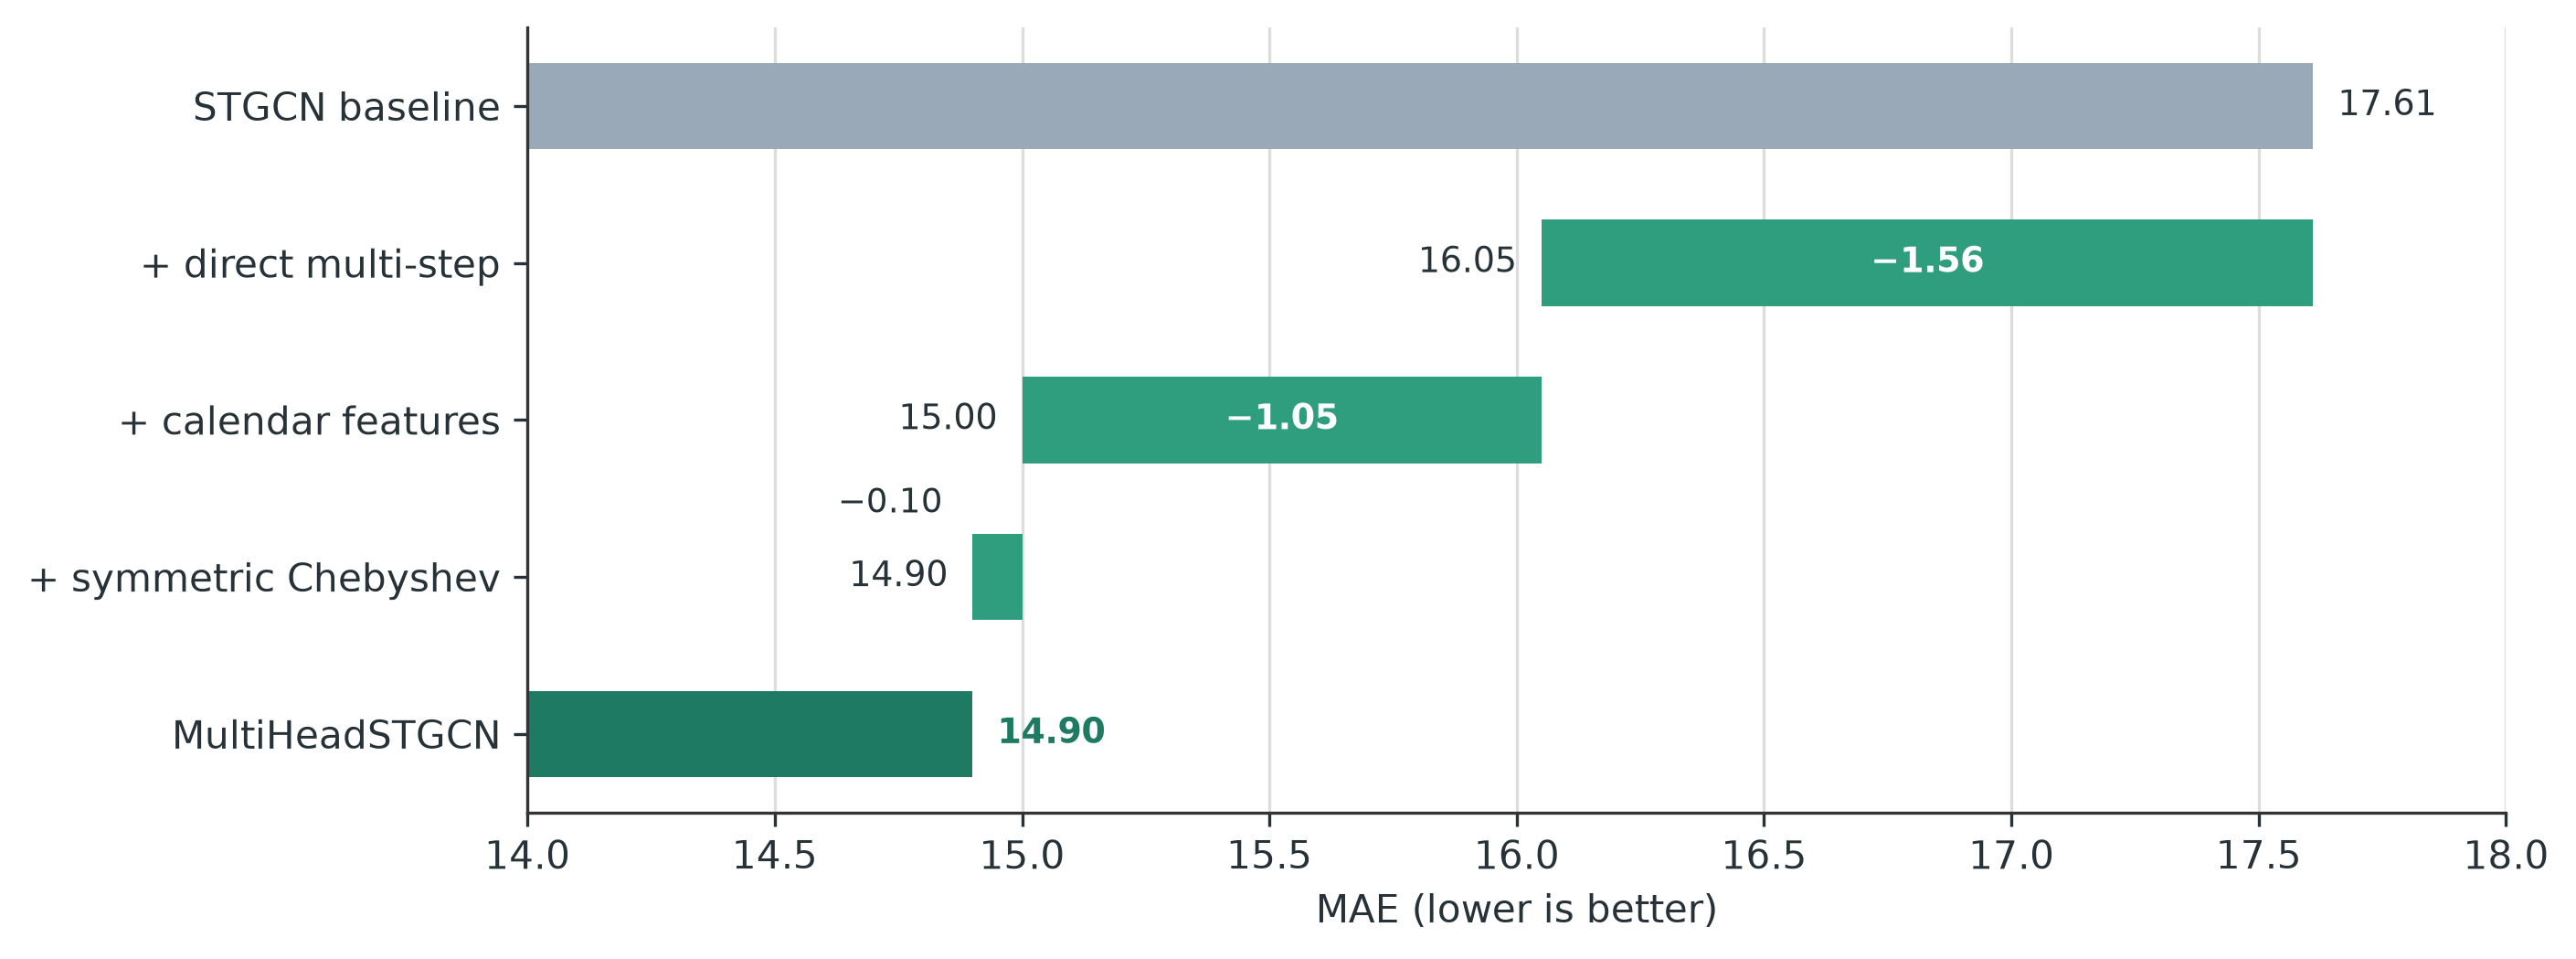
\includegraphics[width=0.9\linewidth]{forecast_ablation.png}
  \caption{Ablation of MultiHeadSTGCN on PEMSD8 traffic flow. Bars show
  absolute MAE; labels give the change from the preceding configuration. The
  x-axis starts at 14 to make the differences visible.}
  \label{fig:ablation}
\end{figure}

In the default-configuration table, MAE is 17.44 for STGCN and 14.84 for
MultiHeadSTGCN, a 14.9\% difference between complete recipes. Under default
configurations the model ranks second, after GWNET (14.648) and ahead of MTGNN
(15.106) and AGCRN (15.612). Under the unified nine-channel input it ranks fourth, after GWNET
(14.365), MTGNN (14.713) and AGCRN (14.777). With five seeds, GWNET's advantage
is 4.22\% (14.1995 versus 14.8256); the paired differences for MTGNN (14.7443)
and AGCRN (14.8913) have confidence intervals that include zero.

\subsection{Unified Input and Multi-Seed Check}\label{sec:results-seeds}

Table~\ref{tab:forecast-unified} reports the unified nine-channel setting. At
seed~0, GWNET is first (14.365), followed by MTGNN (14.713), AGCRN (14.777) and
MultiHeadSTGCN (14.839). The top four were selected by seed-0 test MAE and
re-run with seeds 0--4; this selection is exploratory, and the five-seed
comparison is descriptive rather than a pre-registered confirmatory test. Their
means and paired differences are reported in the same table. GWNET's paired advantage
over MultiHeadSTGCN is −4.22\% (95\% CI −4.98\% to −3.47\%, better on 5/5
seeds). The paired confidence intervals for MTGNN (−0.55\%, CI −1.29\% to
+0.20\%) and AGCRN (+0.44\%, CI −0.38\% to +1.27\%) include zero. Across five
paired seeds, no clear performance difference was established between
MultiHeadSTGCN and MTGNN or AGCRN. These results suggest comparable observed MAE
values, but the limited number of seeds prevents a strong equivalence claim.
GWNET achieved the lowest mean MAE among the four models evaluated across five
seeds. MultiHeadSTGCN also has the smallest seed-to-seed standard deviation
(0.0429). Figure~\ref{fig:multiseed} shows the five-seed means and standard
deviations, and Table~\ref{tab:forecast-horizon} gives the corresponding
15/30/60-minute MAE.

\begin{table}[htbp]
  \centering
  \small
  \caption{Forecasting comparison with unified nine-channel input on PEMSD8
  traffic flow. Seed-0 values cover all eight models; mean ± SD and paired
  differences cover the top four over seeds 0--4.}
  \label{tab:forecast-unified}
  \begin{tabular}{@{}lccc@{}}
    \toprule
    Model & MAE (seed 0) & MAE mean ± SD (seeds 0--4) & \shortstack{Paired diff\\vs MultiHeadSTGCN} \\
    \midrule
    GWNET                & \textbf{14.365} & \textbf{14.1995 ± 0.1022} & −4.22\% ± 0.61\% \\
    MTGNN                & 14.713 & 14.7443 ± 0.0893 & −0.55\% ± 0.60\% \\
    \rowcolor{oursrow}
    MultiHeadSTGCN & 14.839 & 14.8256 ± 0.0429 & -- \\
    AGCRN                & 14.777 & 14.8913 ± 0.0773 & +0.44\% ± 0.67\% \\
    STGCN                & 16.108 & -- & -- \\
    GRU                  & 21.722 & -- & -- \\
    FNN                  & 18.721 & -- & -- \\
    LSTM                 & 25.782 & -- & -- \\
    \bottomrule
  \end{tabular}
  \par\smallskip
  \begin{minipage}{\linewidth}\footnotesize
    \textit{Note.} Bold marks the lowest MAE; the shaded row is the project's
    model. MAE is in vehicles per five-minute interval. All models use nine
    channels: flow, time-of-day (one normalized channel) and day-of-week (seven
    one-hot channels). Mean ± SD describes seed-to-seed variation; the paired
    differences and their 95\% intervals are separate statistics and should not
    be read as standard deviations. Five-seed statistics cover the top four
    only. Negative paired differences mean the baseline has lower MAE than
    MultiHeadSTGCN.
  \end{minipage}
\end{table}

\begin{table}[htbp]
  \centering
  \small
  \caption{MAE by forecast horizon under the unified nine-channel input, mean ±
  SD over seeds 0--4.}
  \label{tab:forecast-horizon}
  \begin{tabular}{@{}lcccc@{}}
    \toprule
    Model & 15 min & 30 min & 60 min & 12-step average \\
    \midrule
    GWNET          & \textbf{13.431 ± 0.084} & \textbf{14.219 ± 0.099} & \textbf{15.465 ± 0.154} & \textbf{14.199 ± 0.102} \\
    MTGNN          & 13.951 ± 0.090 & 14.731 ± 0.091 & 16.035 ± 0.108 & 14.744 ± 0.089 \\
    AGCRN          & 14.137 ± 0.067 & 14.893 ± 0.090 & 16.094 ± 0.121 & 14.891 ± 0.077 \\
    \rowcolor{oursrow}
    MultiHeadSTGCN & 14.233 ± 0.044 & 14.832 ± 0.045 & 15.924 ± 0.068 & 14.826 ± 0.043 \\
    \bottomrule
  \end{tabular}
  \par\smallskip
  \begin{minipage}{\linewidth}\footnotesize
    \textit{Note.} MAE is in vehicles per five-minute interval. The 15, 30 and
    60 minute horizons correspond to output steps 3, 6 and 12. Values are means
    over seeds 0--4; ± is one standard deviation across seeds, not a confidence
    interval.
  \end{minipage}
\end{table}

\begin{figure}[htbp]
  \centering
  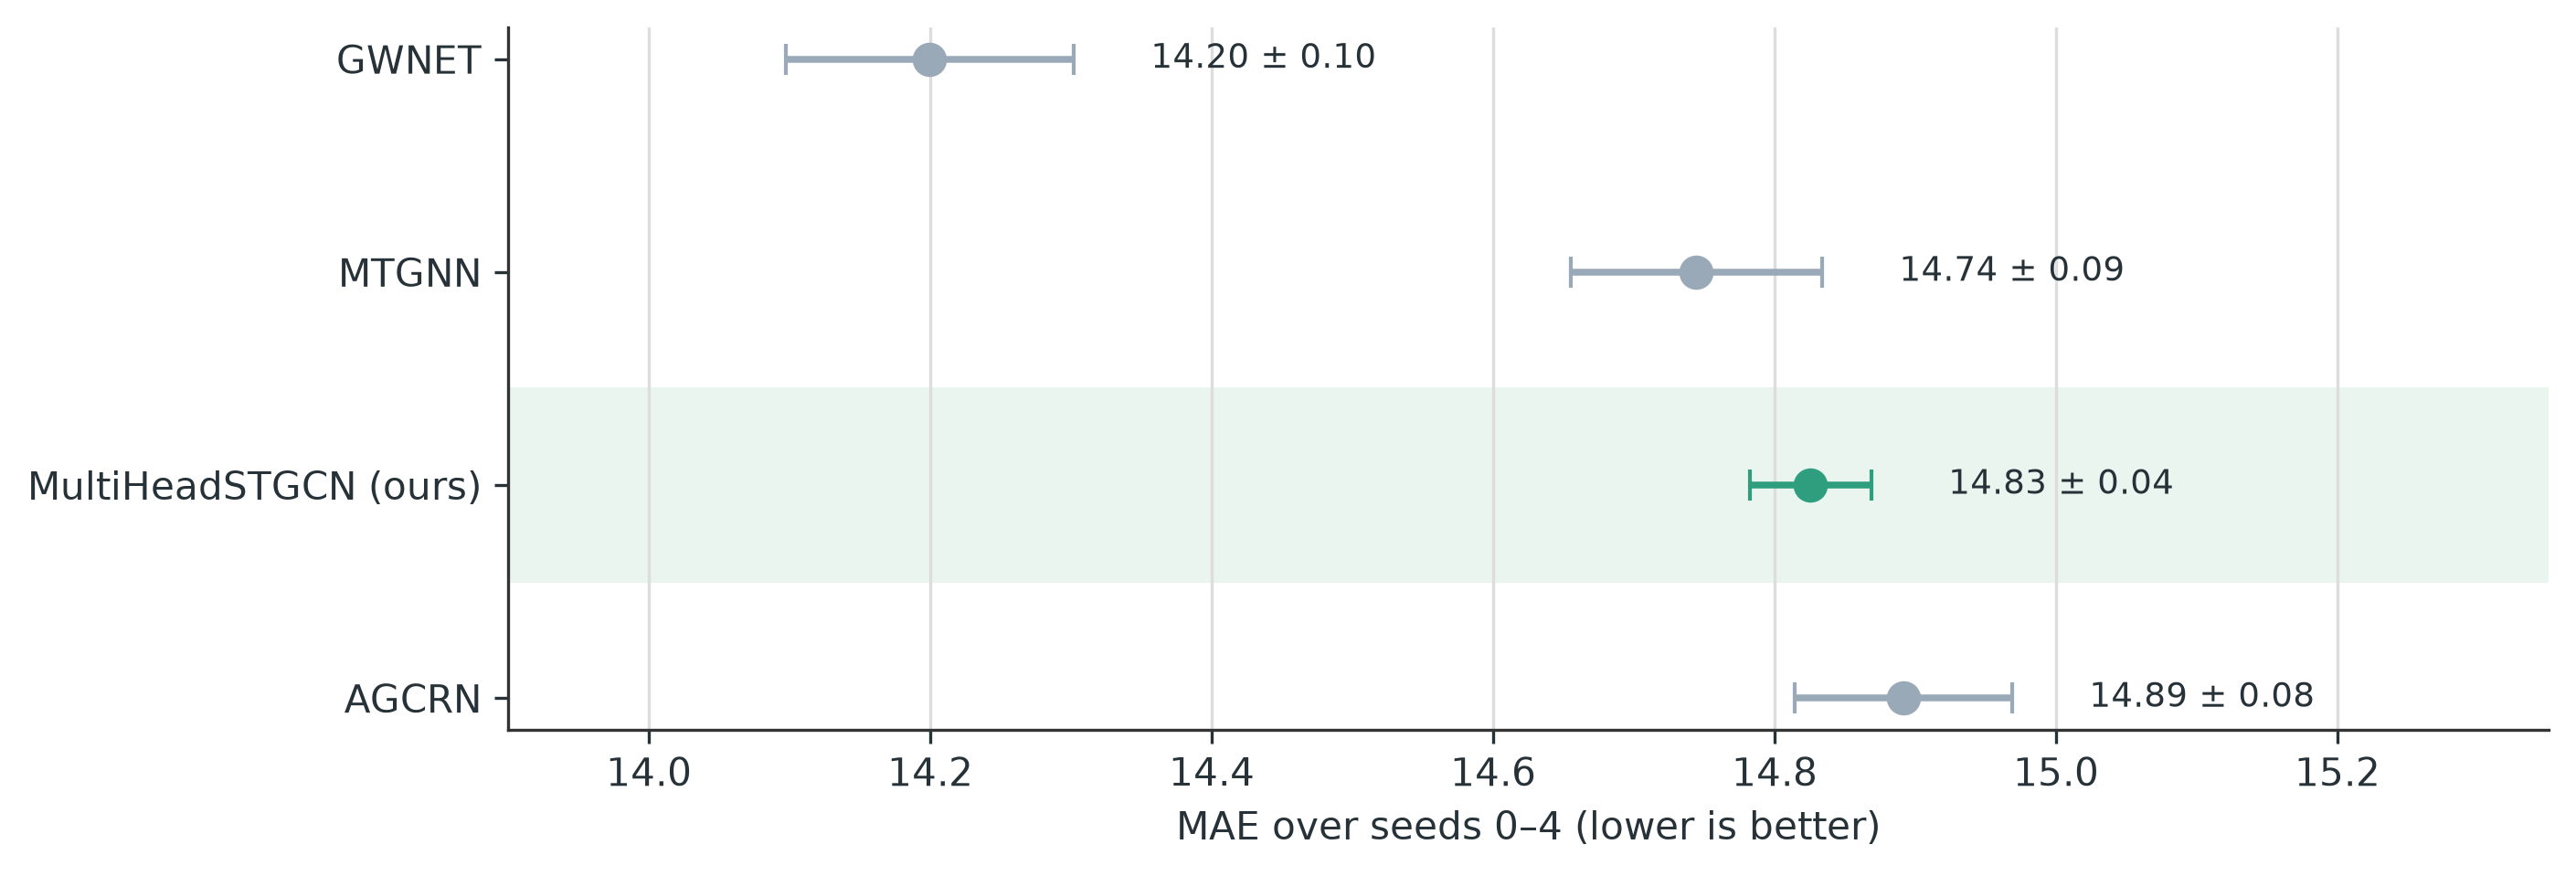
\includegraphics[width=0.9\linewidth]{forecast_multiseed.png}
  \caption{Five-seed MAE on PEMSD8 with unified nine-channel input. Points are
  means over seeds 0--4; error bars show ±1 SD and are not confidence
  intervals.}
  \label{fig:multiseed}
\end{figure}

\subsection{Ablation Findings}\label{sec:results-ablation}

Two ablations are reported. First, calendar features have model-dependent
effects. Adding time-of-day and day-of-week reduces MAE by 11.9\% for FNN,
7.6\% for STGCN, 5.3\% for AGCRN, 2.6\% for MTGNN and 1.9\% for GWNET, and
increases MAE by 10.2\% for GRU and 18.4\% for LSTM. LibCity's RNNs concatenate
all nodes and channels into one vector, so the nine-channel input becomes
1,530-dimensional and is harder to optimize with the default learning rate.

Second, a backbone-matched comparison examines the combined effect of the
changes. MultiHeadSTGCN reduces MAE from 17.61 (STGCN) to about 15.00 (14.8\%),
but because the loss, input features and multi-step strategy also differ, the
reduction cannot be attributed to architecture alone. Multi-target training was
also evaluated; the multi-target variant, which is the only setting that
exercises multiple heads, did not improve flow over the single-target
configuration, so the benchmark uses one target head.

% HUMAN-LTA-SLOT:
% When the human-labeled LTA test set is frozen and evaluated, insert
%     % Human-labeled LTA evaluation.
%
% This file is not included in main.tex yet. To enable it:
%   1. Freeze the human-labeled LTA test set and run the same evaluator used
%      for the teacher-reference results.
%   2. Replace the placeholders below with the new sample size, metrics and
%      interpretation.
%   3. Add % Human-labeled LTA evaluation.
%
% This file is not included in main.tex yet. To enable it:
%   1. Freeze the human-labeled LTA test set and run the same evaluator used
%      for the teacher-reference results.
%   2. Replace the placeholders below with the new sample size, metrics and
%      interpretation.
%   3. Add \input{chapters/05-human-lta} at HUMAN-LTA-SLOT in
%      chapters/05-results-and-analysis.tex.
%
% Inserting this file after Section 5.8 makes it Section 5.9. Existing results
% tables and figures keep their numbers; only later appendix numbering may move.

\subsection{Human-Labeled LTA Evaluation}\label{sec:results-human-lta}

The LTA results in Section~\ref{sec:results-lta} use the frozen YOLO26x teacher
as reference. The human-labeled test set provides an independent accuracy
measurement, with the same four-class evaluator and the same confidence
threshold. It contains [N] images from [cameras and period].

Table~\ref{tab:lta-human} reports the three models on this set.

\begin{table}[htbp]
  \centering
  \small
  \caption{Human-labeled LTA test set ([N] images). mAP@0.5 includes 95\%
  bootstrap intervals.}
  \label{tab:lta-human}
  \begin{tabular}{@{}lccccccc@{}}
    \toprule
    Model & mAP@0.5 & mAP@.5--.95 & Car & Moto. & Bus & Truck & Count MAE \\
    \midrule
    Pretrained YOLO26m & -- & -- & -- & -- & -- & -- & -- \\
    MIO-TCD only       & -- & -- & -- & -- & -- & -- & -- \\
    Joint fine-tuning  & -- & -- & -- & -- & -- & -- & -- \\
    \bottomrule
  \end{tabular}
\end{table}

[Replace this paragraph with the quantitative comparison, confidence intervals
and the effect of replacing the teacher reference. If the conclusion differs
from Section~\ref{sec:results-lta}, state the difference explicitly.]

% Optional figure slot:
% \begin{figure}[htbp]
%   \centering
%   \includegraphics[width=\linewidth]{human_lta_examples.png}
%   \caption{Detection examples on the human-labeled LTA test set.}
%   \label{fig:human-lta-examples}
% \end{figure}
 at HUMAN-LTA-SLOT in
%      chapters/05-results-and-analysis.tex.
%
% Inserting this file after Section 5.8 makes it Section 5.9. Existing results
% tables and figures keep their numbers; only later appendix numbering may move.

\subsection{Human-Labeled LTA Evaluation}\label{sec:results-human-lta}

The LTA results in Section~\ref{sec:results-lta} use the frozen YOLO26x teacher
as reference. The human-labeled test set provides an independent accuracy
measurement, with the same four-class evaluator and the same confidence
threshold. It contains [N] images from [cameras and period].

Table~\ref{tab:lta-human} reports the three models on this set.

\begin{table}[htbp]
  \centering
  \small
  \caption{Human-labeled LTA test set ([N] images). mAP@0.5 includes 95\%
  bootstrap intervals.}
  \label{tab:lta-human}
  \begin{tabular}{@{}lccccccc@{}}
    \toprule
    Model & mAP@0.5 & mAP@.5--.95 & Car & Moto. & Bus & Truck & Count MAE \\
    \midrule
    Pretrained YOLO26m & -- & -- & -- & -- & -- & -- & -- \\
    MIO-TCD only       & -- & -- & -- & -- & -- & -- & -- \\
    Joint fine-tuning  & -- & -- & -- & -- & -- & -- & -- \\
    \bottomrule
  \end{tabular}
\end{table}

[Replace this paragraph with the quantitative comparison, confidence intervals
and the effect of replacing the teacher reference. If the conclusion differs
from Section~\ref{sec:results-lta}, state the difference explicitly.]

% Optional figure slot:
% \begin{figure}[htbp]
%   \centering
%   \includegraphics[width=\linewidth]{human_lta_examples.png}
%   \caption{Detection examples on the human-labeled LTA test set.}
%   \label{fig:human-lta-examples}
% \end{figure}

% here. The template is a separate Section 5.9; existing results tables,
% figures and section numbers stay unchanged. Keep the teacher-reference results in 5.2 as
% a separate proxy unless the new labels are intended to replace them.

\section{Discussion}\label{sec:discussion}

\subsection{Detection Performance}\label{sec:discussion-detection}

On MIO-TCD, where human labels are available, fine-tuning yields a substantial
improvement on the evaluated dataset: mAP@0.5 rises from 0.430 to 0.720 and the
gain is stable across scene groups. On the LTA images the reference is the
YOLO26x teacher, and the joint model reaches 0.638 at the batch-inference
resolution, close to the pretrained model's 0.660 and well above MIO-only
training at 0.201. Joint training improves agreement on the Singapore validation
set while retaining the accuracy gained from MIO-TCD. The human-labeled MIO-TCD
test set provides the accuracy benchmark, and the LTA figures measure
cross-domain agreement with the teacher.

\subsection{Camera Filter and Congestion Levels}\label{sec:discussion-congestion}

The camera filter shows that fixed scenes allow a simple, transparent correction
of a learned detector: it removes 2.0\% of boxes and raises precision by 1.7
points on unseen human-labeled images, without retraining. The gain is small
because most errors on LTA frames are missed vehicles, which a filter cannot
recover; recall, not precision, limits counting on these cameras.

For congestion, a stacked combination of a trained detector, classical image
processing and a zero-shot vision-language model agrees with 74.3\% of held-out
human labels, and recognizes the congested level with precision 0.88 and recall
0.84. Its 2.0-point gain over the detector count lies within the uncertainty of a
400-frame test, so the result supports the method as a working estimate rather
than showing that combining voters is necessary. The main difficulty is the
moderate level, which is usually rated free-flowing, the boundary where the
visual difference between levels is smallest. Because every design choice was
made on practice labels and the test labels were used once, 74.3\% is a fair
estimate for new frames from the same cameras and period. The levels are a
visual judgement of the outlined road, not a calibrated flow or speed, so they do
not close the integration gap described in Section~\ref{sec:method-integration}.

\subsection{Forecasting Performance}\label{sec:discussion-forecasting}

The forecasting module was selected through the common-protocol comparison.
GWNET is the best-performing model under the evaluated setting. Across five
paired seeds, no clear difference was established between MultiHeadSTGCN and
MTGNN or AGCRN, and the limited number of seeds does not support an equivalence
claim. The backbone-matched configuration lowers MAE relative to STGCN by about
14.8\% in the staged ablation and by 14.9\% in the default-configuration
benchmark, but these comparisons also change inputs, loss and training strategy;
they should not be read as an isolated architectural effect. Under both native
and unified inputs, GWNET retains the lowest MAE in this benchmark.

\subsection{Module Integration}\label{sec:discussion-integration}

The detection and forecasting modules are part of one prototype and operate on
different data domains. The detection module consumes camera images; the
forecasting module consumes road-network time series. The workbench reads both
sets of outputs and labels their sources, so a user can inspect the monitoring
view and the forecast view with the corresponding data source identified. The
separation follows the available data coverage; both modules remain part of the
same prototype. Section~\ref{sec:method-integration} defines the interface for a
connected system, and Section~\ref{sec:discussion-roadmap} discusses the
implications of moving from the prototype to that system.

\subsection{Implications for Future Integration}\label{sec:discussion-roadmap}

Section~\ref{sec:method-integration} defines the data interface; the main
implication is that integration is a measurement problem before it is a modeling
problem. Camera counts must be calibrated against a trusted volume source and
aggregated to a fixed interval, because a detector count per still image is not a
flow series. The same locations also need time-aligned flow, and ideally
occupancy and speed, over weeks or months. Where the existing view is too distant
or poorly lit, close-range cameras or dedicated sensors are the practical way to
obtain those measurements.

A second implication concerns model transfer. A forecasting model trained on
PEMSD8 learns California sensor dynamics; applying it to a Singapore series
would require retraining and a new evaluation on the local split. Detection
counts could enter as an exogenous variable, but only after calibration and
timestamp alignment. These steps define the work that remains before the
workbench can present one local monitoring-and-forecasting workflow rather than
two source-labeled views.

\subsection{Limitations and Scope}\label{sec:discussion-limitations}

The reported system is a time-bounded prototype and pipeline design. It
demonstrates the processing chain and evaluation protocol. An operational
LTA-to-Singapore system would require calibrated sensing and longer data
collection.

\begin{itemize}
  \item LTA results use the YOLO26x pseudo-labels as reference, so they measure
        agreement with the teacher, and the student inherits the teacher's
        missed motorcycles and false positives. Human-labeled MIO-TCD provides
        the accuracy benchmark.
  \item Nighttime LTA frames are difficult to annotate even for humans:
        vehicles are small, poorly lit and often blurred. Teacher labels and
        human labels collected at night are the least reliable reference.
  \item LTA agreement depends on inference resolution: the joint model leads at
        960 pixels and the pretrained model at 1280 pixels.
  \item Scene groups provide a content-based proxy for camera identity, so the
        MIO-TCD test set can retain residual same-camera overlap. In an audit of
        40 test images, each paired with its most similar training image, a
        preliminary visual review found 9 same-camera pairs. The test score
        therefore describes a mix of seen and unseen cameras, not generalization
        to new cameras.
  \item MIO-TCD is evaluated on a filtered four-class subset with a
        project-defined class mapping.
  \item The workbench risk ranking is a threshold-based indicator defined on
        predicted speed. It supports comparative inspection but has not been
        validated against an independent congestion label.
  \item The camera filter and congestion evaluations rely on a single
        annotator. The congestion test set has 50 frames per camera, and two
        weeks give each weekday only two or three days, so per-camera and
        per-slot figures are uncertain.
  \item Congestion is judged only inside the calibrated detection zones, not
        along the whole road, and the zones and road regions must be
        recalibrated if a camera is moved or re-aimed.
  \item The LTA images are still images at ten-minute intervals. They support
        vehicle counts per frame but not continuous passage counts at a point.
        A PEMSD8-style flow series would require continuous video, tracking,
        lane or region calibration, and validation against a loop or radar
        sensor.
  \item Full local integration requires additional IoT measurements (loop
        detectors, radar, LiDAR or traffic counters) at the camera locations to
        provide calibrated flow, occupancy and speed. Close-range road cameras
        are an alternative when the existing camera geometry or lighting is
        unfavorable.
\end{itemize}

\section{Conclusion}\label{sec:conclusion}

This project developed a modular prototype for traffic monitoring and
short-term forecasting, comprising a vehicle recognition module, a traffic
forecasting module and a web-based workbench. The system evaluates visual
recognition and sensor-based forecasting on their respective data domains while
keeping the boundary between those domains explicit.

For vehicle recognition, fine-tuning improved mAP@0.5 from 0.430 to 0.720 on the
human-labeled MIO-TCD test subset. Joint training with target-domain
pseudo-labels also improved agreement with the teacher model on the LTA
validation set relative to MIO-TCD-only training. On 63 human-labeled LTA
images, the joint model matched the pretrained detector in mAP@0.5 (0.478 versus
0.467) while reducing counting error and raising recall. These findings show the
value of traffic-specific adaptation on the benchmark, while adaptation to the
Singapore viewpoint is only partly solved; nighttime frames remain the least
reliable part of the evaluation.

Two further components extend the recognition output. A per-camera filter, calibrated by
hand, raised precision on 63 human-labeled LTA images from 0.816 to 0.833 at a
small cost in recall. A stacked ensemble of the detector count, background
differencing and zero-shot CLIP rated all 15,316 frames as free-flowing,
moderate or congested, agreeing with 74.3\% of 400 held-out human labels. The
resulting heatmaps show recurring congestion on the Causeway and Second Link
cameras at weekday peaks and on Saturdays.

For traffic forecasting, eight models were evaluated on PEMSD8 under native and
unified-input configurations. GWNET achieved the lowest MAE among the evaluated
configurations, while MultiHeadSTGCN produced competitive results without a
clearly established difference from MTGNN or AGCRN across five seeds. The staged
ablation associated direct multi-step prediction and calendar features with
substantial reductions in MAE relative to the reference STGCN configuration.
Because input features, loss and training strategy also changed, these
reductions cannot be attributed to architecture alone.

The workbench presents the monitoring and forecasting outputs in one interface,
with source labels, historical replay and a threshold-based risk indicator. The
two modules currently operate on different data domains and do not constitute an
end-to-end Singapore forecasting pipeline. Future integration requires
calibrated, time-aligned local measurements, retraining on the local series and
evaluation of the resulting workflow. Overall, the project establishes a modular
implementation and an experimental basis for that next stage.


\clearpage
\begin{sloppypar}
\printbibliography[heading=bibintoc,title={References}]
\end{sloppypar}

\clearpage
\appendix
\clearpage
\section{Declaration of AI Tool Usage}\label{app:ai-declaration}

Table~\ref{tab:ai-declaration} declares all use of AI tools in the preparation
of this report, as required by the school's AI policy. All quantitative results
reported in this report were produced by executing the project's own code and
reading its outputs.

\begin{table}[htbp]
  \centering
  \footnotesize
  \singlespacing
  \caption{Declaration of AI tool usage.}
  \label{tab:ai-declaration}
  \begin{tabularx}{\textwidth}{@{}>{\raggedright\arraybackslash}p{3.2cm}>{\raggedright\arraybackslash}p{4.4cm}X@{}}
    \toprule
    AI Tool & Purpose & How the output was used \\
    \midrule
    Claude Code (Anthropic) &
    Debugging and optimization of parts of the code; Chinese--English translation &
    Assisted with implementing and checking code and translating the English document. The authors reviewed and confirmed all content and results. \\
    Codex (OpenAI) &
    Debugging and optimization of parts of the code &
    Assisted with implementing and checking code and provided code revision suggestions. The authors reviewed and integrated the suggestions. \\
    \bottomrule
  \end{tabularx}
\end{table}

\noindent Author confirmation: The research design, experiment execution, data
interpretation and conclusions in this report were completed by the authors. The
AI tools listed above were used for code debugging and optimization and for
translation; they did not replace the authors'
research judgments. All quantitative results were produced by executing the
project's own code and reading its outputs. All external literature cited in
the main text is listed in the references.


\end{document}
